\documentclass{article}
\usepackage{graphicx}
\usepackage{float}  
\usepackage[utf8]{inputenc}
\usepackage[includeheadfoot, margin=1em,headheight=2em]{geometry}
\usepackage{titling}
\usepackage{hyperref}
\geometry{a4paper, left=2cm, right=2cm, top=2cm, bottom=2cm}
\usepackage{graphicx}
\providecommand{\versionnumber}{1.0.0}
\usepackage{enumitem}
\usepackage{svg}
\usepackage[italian]{babel}
\usepackage{array}
\newcolumntype{P}[1]{>{\centering\arraybackslash}p{#1}}
\renewcommand{\arraystretch}{1.5} % Default value: 1
\setlength{\droptitle}{-6em}
\usepackage{capt-of}
\usepackage{url}
\usepackage{setspace}

% Font
\usepackage[defaultfam,tabular,lining]{montserrat}
\usepackage[T1]{fontenc}
\renewcommand*\oldstylenums[1]{{\fontfamily{Montserrat-TOsF}\selectfont #1}}

%custom bold 
\usepackage[outline]{contour}
\usepackage{xcolor}
\newcommand{\custombold}{\contour{black}}

%table colors
\usepackage{color, colortbl}
\definecolor{Blue}{rgb}{0.51,0.68,0.79}
\definecolor{LightBlue}{rgb}{0.82,0.87,0.90}
\definecolor{LighterBlue}{rgb}{0.93,0.95,0.96}

\usepackage{caption}
\captionsetup[figure]{labelformat=empty}

%Header
\usepackage{fancyhdr, xcolor}
\pagestyle{fancy}
\let\oldheadrule\headrule% Copy \headrule into \oldheadrule
\renewcommand{\headrule}{\color{Blue}\oldheadrule}% Add colour to \headrule
\renewcommand{\headrulewidth}{0.2em}
\fancyhead[L]{Specifica Tecnica}
\fancyhead[C]{Cybersorceres}
\fancyhead[R]{versione \versionnumber}

\renewcommand{\labelitemiii}{$\cdot$}

\title{\Huge{\textbf{Specifica Tecnica}}\vspace{-1em}}
\author{CyberSorcerers Team}
\date{}
\begin{document}
\maketitle
\vspace{-3em}
\begin{figure}[h]
  \centering
  
\includegraphics[width=6cm, height=6cm]{documenti/logo rotondo.png}
  \label{fig:immagine}
\end{figure}

\begin{center}
    \begin{tabular}{|l c c|}
    \hline
        \rowcolor{Blue} 
        \textbf{Informazioni sul documento} & &\\ [1 ex]
        \hline
        \rowcolor{LighterBlue}
        Destinatari: & Prof Tullio Vardanega & Prof Riccardo Cardin\\ [1 ex]
        \hline
        \rowcolor{LightBlue}
        G al pedice: & Consultare il Glossario & \\ [1 ex]
        \hline
    \end{tabular}
\end{center}


\vspace{6em}
\begin{center}
    \begin{tabular}{|P{24em}|}
    \hline
        \rowcolor{Blue}
        \textbf{Membri del team:}\\
        \hline
        \rowcolor{LighterBlue}
        \custombold{Sabrina Caniato}\\
        \hline
        \rowcolor{LightBlue}
        \custombold{Giulia Dentone}\\
        \hline
        \rowcolor{LighterBlue}
        \custombold{Nicola Lazzarin}\\
        \hline
        \rowcolor{LightBlue}
        \custombold{Giovanni Moretti}\\
        \hline
        \rowcolor{LighterBlue}
        \custombold{Andrea Rezzi}\\
        \hline
        \rowcolor{LightBlue}
        \custombold{Samuele Vignotto}\\
        \hline
    \end{tabular}
\end{center}

    
\newpage

\textbf{Registro dei Cambiamenti - Changelog\textsubscript{G}}
\begin{center}
\begin{tabular}{P{4em} P{6em} P{8em} P{8em} P{10em}} 
  \rowcolor{Blue}
    \custombold{Versione} & \custombold{Data} & \custombold{Autore} &
    \custombold{ Verificatore} & \custombold{Dettaglio}\\
    \rowcolor{LighterBlue}
    1.0.0 & 28/05/2024 & Giulia Dentone & Samuele Vignotto & Verifica finale documento.\\
    \rowcolor{LightBlue}
    0.8.0 & 27/05/2024 & Andrea Rezzi & Giovanni Moretti & Stesura della sezione 'Architettura Back-end'.\\
    \rowcolor{LighterBlue}
    0.7.0 & 27/05/2024 & Samuele Vignotto & Giulia Dentone & Stesura della sezione 'Architettura front-end Login e Password'.\\
    \rowcolor{LightBlue}
    0.6.0 & 27/05/2024 & Sabrina Caniato & Giovanni Moretti & Stesura della sezione 'Architettura Front-End'.\\
    \rowcolor{LighterBlue}
    0.5.0 & 26/05/2024 & Sabrina Caniato & Giulia Dentone & Stesura della sezione 'Architettura Libreria'.\\
    \rowcolor{LightBlue}
    0.4.0 & 26/05/2024 & Giovanni Moretti & Sabrina Caniato & Stesura della sezione 'Architettura Plugin'.\\
    \rowcolor{LighterBlue}
    0.3.0 & 25/05/2024 & Sabrina Caniato & Andrea Rezzi & Stesura della sezione 'Schema del Database'.\\
    \rowcolor{LightBlue}
    0.2.0 & 23/05/2024 & Samuele Vignotto & Giovanni Moretti & Stesura della sezione 'Requisiti soddisfatti'.\\
    \rowcolor{LighterBlue}
    0.1.1 & 23/05/2024 & Giulia Dentone & Sabrina Caniato & Stesura della sezione 'Tecnologie'.\\
    \rowcolor{LightBlue}
    0.0.1 & 03/05/2024 & Giulia Dentone & Samuele Vignotto &  Definizione struttura del documento e scheletro delle sezioni. Scrittura introduzione ed obiettivi delle diverse sezioni.\\
\end{tabular}
\end{center}
\newpage
\tableofcontents
\listoffigures
\listoftables
\newpage

\section{Introduzione}
\subsection{Scopo del documento}
Questo documento ha lo scopo di delineare e giustificare le decisioni architetturali prese durante le fasi di progettazione e sviluppo del prodotto. Sono presentati i diagrammi dei componenti React e dei pacchetti per illustrare le scelte dei pattern architetturali adottati per realizzare la struttura finale del prodotto. Inoltre, viene fornita una sezione dedicata ai requisiti soddisfatti dal team, offrendo così una panoramica completa dello stato di avanzamento del lavoro.
\subsection{Scopo del prodotto}
L'azienda proponente ha richiesto la creazione di una web app\textsubscript{G} che, tramite l'uso di IA\textsubscript{G} (in questo caso ChatGPT4 e Bedrock) è in grado di creare epic user stories\textsubscript{G} a partire dalle richieste del cliente e confrontarle con il codice sviluppato in modo da informare il cliente dello stato di avanzamento dello sviluppo del prodotto. Inoltre deve essere possibile, sia per il Project Manager\textsubscript{G}, sia per il cliente rilasciare dei feedback (nel primo caso riguardanti l'adeguatezza delle stories, nel secondo caso riguardanti il prodotto finale) al fine di migliorare l'IA\textsubscript{G}. È inoltre richiesta un' analisi comparativa tra le due IA\textsubscript{G} utilizzate e lo sviluppo di un plug-in\textsubscript{G} utile agli sviluppatori e al Project Manager\textsubscript{G}.

\subsection{Glossario}
Alcuni termini presenti nel documento potrebbero essere ambigui, pertanto verranno inseriti nel Glossario v.1.0.0. La loro presenza all'interno di esso sarà indicata tramite una G maiuscola a pedice.

\section{Riferimenti}
\subsection{Riferimenti normativi}
\begin{itemize}
    \item Capitolato \textbf{C7 - ChatGPT vs BedRock developer Analysis}
    \\ \\
       \href{https://github.com/CyberSorceres/CyberSorceresRepository}{https://github.com/CyberSorceres/CyberSorceresRepository} 
    \item Norme del way of working v 1.0.0
    \item Regolamento del progetto didattico \\ \\ \href{https://www.math.unipd.it/~tullio/IS-1/2023/Dispense/PD2.pdf} 
    {https://www.math.unipd.it/~tullio/IS-1/2023/Dispense/PD2.pdf}
\end{itemize}
\subsection{Riferimenti informativi}
\begin{itemize}
    \item Slide del corso di Ingegneria del Software - Analisi dei requisiti \\ \\
    \href{https://www.math.unipd.it/~tullio/IS-1/2023/Dispense/T5.pdf}{https://www.math.unipd.it/~tullio/IS-1/2023/Dispense/T5.pdf}
    \item Slide del corso di Ingegneria del Software - Progettazione e programmazione: Diagrammi delle classi \\ \\
\href{https://www.math.unipd.it/~rcardin/swea/2023/Diagrammi%20delle%20Classi.pdf}{https://www.math.unipd.it/~rcardin/swea/2023/Diagrammi\%20delle\%20Classi.pdf}
    \item Slide del corso di Ingegneria del Software - Solid Programming \\ \\
\href{https://www.math.unipd.it/~rcardin/swea/2021/SOLID\%20Principles\%20of\%20Object-Oriented\%20Design_4x4.pdf}{\texttt{https://www.math.unipd.it/~rcardin/swea/2021/SOLID\%20Principles\%20of\%20Object-Oriented\%20Design\_4x4.pdf}}
\end{itemize}
\subsection{Riferimenti tecnici}
\begin{itemize}
\item Documentazione di React \\ \href{ https://react.dev/}{ https://react.dev/}
\item Documentazione di Typescript \\ \href{https://www.typescriptlang.org/docs/}{https://www.typescriptlang.org/docs/}
\item Documentazione di MongoDB \\ \href{https://www.mongodb.com/docs/}{https://www.mongodb.com/docs/}
\item Documentazione di Amazon AWS \\ \href{https://docs.aws.amazon.com/it_it/}{https://docs.aws.amazon.com/it\_it/}
\item Serverless Microservice Patterns \\\href{https://medium.com/@jeremydaly/serverless-microservice-patterns-for-aws-6dadcd21bc02}{https://medium.com/@jeremydaly/serverless-microservice-patterns-for-aws-6dadcd21bc02}
\item Aws Reference Architecture Diagrams \\ \href{https://aws.amazon.com/it/architecture/reference-architecture-diagrams}{https://aws.amazon.com/it/architecture/reference-architecture-diagrams}
\item React design patterns \\ \href{https://refine.dev/blog/react-design-patterns/}{https://refine.dev/blog/react-design-patterns/}
\end{itemize}

\section{Tecnologie}
In questa sezione è presente una panoramica generale delle tecnologie necessarie per la realizzazione del prodotto (in particolare del front-end, back-end,databse e plugIn), gli strumenti e le librerie utilizzate per lo sviluppo, il testing e la distribuzione.

\subsection{Tecnologie per la codifica}

\begin{center}
\begin{tabular}{|P{8em}|P{18em}|P{5em}|}
\hline
\rowcolor{Blue}
Tecnologia & Descrizione & Versione \\
\hline
\rowcolor{LighterBlue}
\multicolumn{3}{|c|}{Linguaggi} \\
\hline
\rowcolor{LightBlue}
HTML & Linguaggio di markup per delineare la struttura delle pagine e definire i componenti dell'interfaccia. & 5 \\
\hline
\rowcolor{LighterBlue}
CSS & Linguaggio per la gestione dello stile degli HTML & 3 \\
\hline
\rowcolor{LightBlue}
Typescript & Superset di JavaScript per utilizzare tipizzazione & 5.0.x \\
\hline
\rowcolor{LighterBlue}
\multicolumn{3}{|c|}{Framework} \\
\hline
\rowcolor{LightBlue}
React & Libreria grafica per lo sviluppo front-end che permette di gestire le unità grafiche in maniera modulare& 18.0.x \\
\hline
\rowcolor{LighterBlue}
\multicolumn{3}{|c|}{Servizi e strumenti} \\
\hline
\rowcolor{LightBlue}
Node.js & Ambiente di runtime open-source per l'esecuzione di codice JavaScript lato
server tramite appositi script. & 19.0.x \\
\hline
\rowcolor{LighterBlue}
NPM & Gestore dell'installazione della gestione dei pacchetti utilizzati in TypeScript e nell'ambiente di esecuzione Node.js. & 3 \\
\hline
\rowcolor{LightBlue}
AWS Cognito & Servizio di gestione dell'autenticazione. & 2023-16-02\\
\hline
\rowcolor{LighterBlue}
AWS MongoDB & Servizio di database non relazionale gestito in modo scalabile. & 2019-11-21\\
\hline
\rowcolor{LightBlue}
AWS Lambda & Servizio che consente di eseguire codice in maniera serverless, garantendo la scalabilità automatica durante l'esecuzione. & 2023-03-16 \\
\hline
\rowcolor{LighterBlue}
AWS API Gateway & Servizio di gestione (creazione, pubblicazione e protezione) delle API. & 2023-04-06\\
\hline
\rowcolor{LightBlue}
Git & Sistema di controllo del versionamento e della gestione del codice. & 2.4.x\\
\hline
\end{tabular}
\captionof{table}{Tabella delle tecnologie per la codifica}
\label{tab:teccod}
\end{center}


\subsection{Tecnologie per l'analisi del codice}
\begin{center}
\begin{tabular}{|P{8em}|P{18em}|P{5em}|}
\hline
\rowcolor{Blue}
Tecnologia & Descrizione & Versione \\
\rowcolor{LighterBlue}
\hline
\multicolumn{3}{|c|}{Analisi statica} \\
\hline
\rowcolor{LightBlue}
Prettier & Strumento di formattazione del codice che mantiene lo stile di
codifica coerente e leggibile. & 3.0.x \\
\hline
\rowcolor{LighterBlue}
ViTest & Framework di test per TypeScript che permette la creazione di mock e il testing del codice in modo asincrono. & 1.6.0\\ 
\rowcolor{LightBlue}
\hline
\multicolumn{3}{|c|}{Analisi dinamica} \\
\hline
\rowcolor{LighterBlue}
React Testing Library & Libreria di test che consente di testare il comportamento dei componenti React da una prospettiva degli utenti finali. & 14.0.x \\
\hline
\rowcolor{LightBlue}
Github Actions & Piattaforma di integrazione e distribuzione continua per automatizzare flussi di lavoro software come build, test e deployment direttamente su GitHub. & / \\
Postman & è un'applicazione software utilizzata per il testing delle API & 10.16\\
\hline
\end{tabular}
\end{center}


\section{Architettura}
Nella fase di progettazione è stata scelta un'architettura a microservizi come la più conforme alle carateristiche di funzionamento e strutturali delle tecnologie AWS, soprattutto API Gateway. Inoltre è quella che consente nel nostro caso la comunicazione  per consentire la comunicazione tra le diverse componenti, considerando anche la presenza di un plugIn. Dati i requisiti del nostro progetto, abbiamo deciso che non fosse adeguato adottare un'unica struttura architetturale per l'intera l'infrastruttura. Abbiamo suddiviso il sistema in tre parti principali: 
\begin{itemize}
    \item Front-end: la parte client dell'applicazione eseguibile localmente su qualsiasi browser.
    \item Back-end: utilizza le tecnologie AWS (listate nella sezione 3.1), con l'interazione tramite NodeJS lato client e la comunicazione con il plugIn. 
    \item PlugIn: comunica con il back-end grazie ad una libreria sviluppata dal team.
\end{itemize}
La comunicazione tra le diverse parti avviene attraverso l'uso di API Gateway.

 \begin{figure}[H]
      \centering
      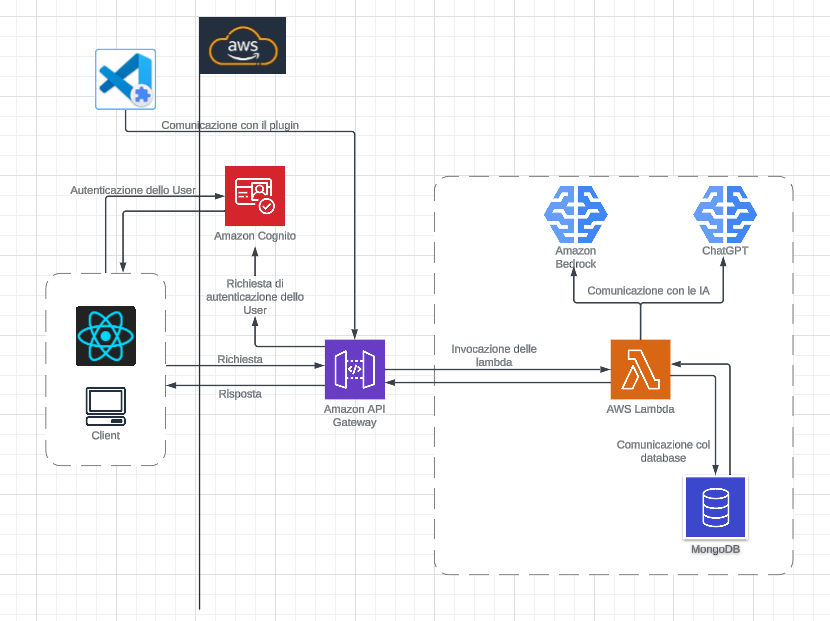
\includegraphics{documenti/grafici/schema backend.png}
      \caption{Schema dei componenti}
      \label{fig: backendscheme}
    \end{figure}

\subsection{Architettura front-end}
L'architettura del frontend\textsubscript{G} della nostra applicazione è stata progettata per essere modulare e scalabile, utilizzando tecnologie moderne e seguendo i migliori pattern di design per garantire un'alta manutenibilità e facilità di sviluppo. Il frontend\textsubscript{G} è realizzato utilizzando React\textsubscript{G} e TypeScript\textsubscript{G}, che offrono un ambiente robusto per la costruzione di interfacce utente interattive e reattive.
\subsubsection{Pattern utilizzati}
Per garantire un'architettura modulare e mantenibile, sono stati utilizzati diversi pattern di design tipici dello sviluppo con React\textsubscript{G}:
\begin{itemize}
    \item \custombold{Controlled Components}: I valori di input dei componenti vengono gestiti direttamente e passati dai componenti "parent" ai componenti "children" sotto forma di props, garantendo che i dati siano costanti tra tutti i componenti.
    \item \custombold{Presentational and Container Components}: La logica di presentazione è separata dalla logica di business, realizzando componenti React\textsubscript{G} che si occupano di renderizzare una vista e utilizzandoli all’interno di un componente unico.
    \item \custombold{React Hooks}: Utilizzati per gestire lo stato dell’applicazione in modo efficiente e per aggiornare dinamicamente le informazioni. Sono stati utilizzati hooks\textsubscript{G} standard di React (useState, useEffect, useContext) e hooks\textsubscript{G} personalizzati in base alle esigenze delle singole viste e componenti (useLoaderData, useNavigate).
    \item \custombold{Provider}: Racchiude l’intera applicazione per fornire il componente di autenticazione a tutti i componenti, semplificando la gestione dell’autenticazione e delle autorizzazioni.
    \item \custombold{Conditional Rendering}: Consente di mostrare un contenuto diverso a seconda del ruolo dell’utente, rendendo l’interfaccia più dinamica e adattabile.
    \item \custombold{Compound Components}: Utilizzati per modularizzare le singole componenti, creando una gerarchia padre-figlio dove il componente padre contiene uno o più componenti figlio, specializzando la gestione dei dati e la personalizzazione dell’interfaccia utente in modo centralizzato.
\end{itemize}
\subsubsection{Diagrammi delle classi}
La sezione seguente descrive le singole pagine per i vari utenti utilizzando la sintassi UML\textsubscript{G} e una descrizione testuale appropriata. Questo serve a rendere ogni scelta progettuale del gruppo Cybersorceres chiara e facilmente interpretabile durante il periodo di sviluppo.

\subsection{App}
\begin{figure}[H]
    \centering
    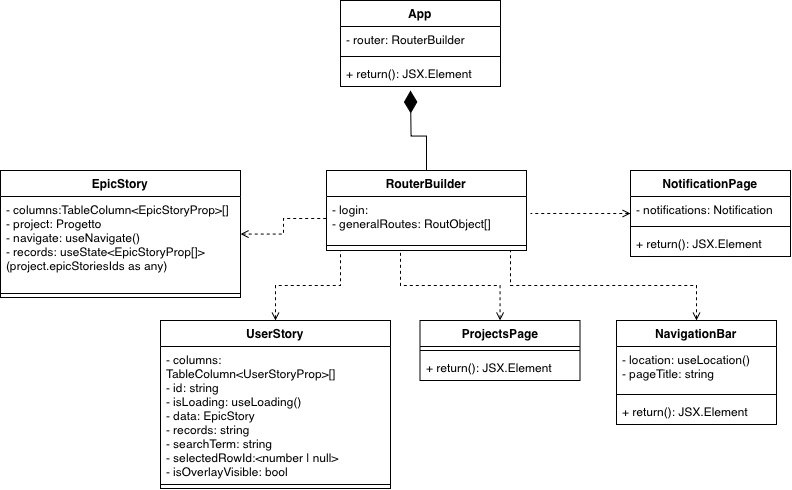
\includegraphics[width=1\textwidth, height=400pt]{documenti/imgUMLFrontend/App.jpg}
    \caption{UML App}
    \label{fig:uml-App}
\end{figure}
\subsection{App}

\subsubsection*{Descrizione}
Il componente \textbf{App} costituisce il componente principale dell'applicazione. È responsabile per l'inizializzazione del contesto API e la gestione del routing.

\subsubsection*{Variabili di Stato}
\begin{itemize}
    \item \textbf{api}: un'istanza dell'oggetto API che gestisce le richieste verso il server.
\end{itemize}

\subsubsection*{Funzioni Principali}
\begin{itemize}
    \item \textbf{createAPI}: funzione per la creazione dell'oggetto API con il token memorizzato nel localStorage, se disponibile.
\end{itemize}

\subsubsection*{Rendering}
Il componente \textbf{App} rende il contesto API all'interno di un \texttt{APIContext.Provider}, che è accessibile a tutti i componenti all'interno dell'applicazione. Inoltre, utilizza il componente \texttt{RouterProvider} per fornire il router creato tramite \texttt{createBrowserRouter}.

\subsection*{RouterBuilder}

\subsubsection*{Descrizione}
La funzione \textbf{RouterBuilder} è responsabile per la costruzione delle route dell'applicazione. Utilizza l'oggetto API fornito come argomento per determinare le route disponibili e configurare i loro componenti e loader.

\subsubsection*{Parametri}
\begin{itemize}
    \item \textbf{api}: un'istanza dell'oggetto API che gestisce le richieste verso il server.
\end{itemize}

\subsubsection*{Variabili Locali}
\begin{itemize}
    \item \textbf{login}: una variabile di stato che indica se l'utente è autenticato.
    \item \textbf{generalRoutes}: un array di oggetti che rappresentano le route generali dell'applicazione.
\end{itemize}

\subsubsection*{Funzioni Principali}
\begin{itemize}
    \item \textbf{setLogin}: funzione per impostare lo stato di autenticazione dell'utente.
\end{itemize}

\subsubsection*{Rendering}
La funzione \textbf{RouterBuilder} restituisce un array di route che definiscono la struttura dell'applicazione. Queste route includono le route generali e i loro componenti corrispondenti. Le route vengono renderizzate all'interno di un componente \texttt{Suspense}, che fornisce un fallback durante il caricamento asincrono delle route.

\subsection{Login}
\begin{figure}[H]
    \centering
    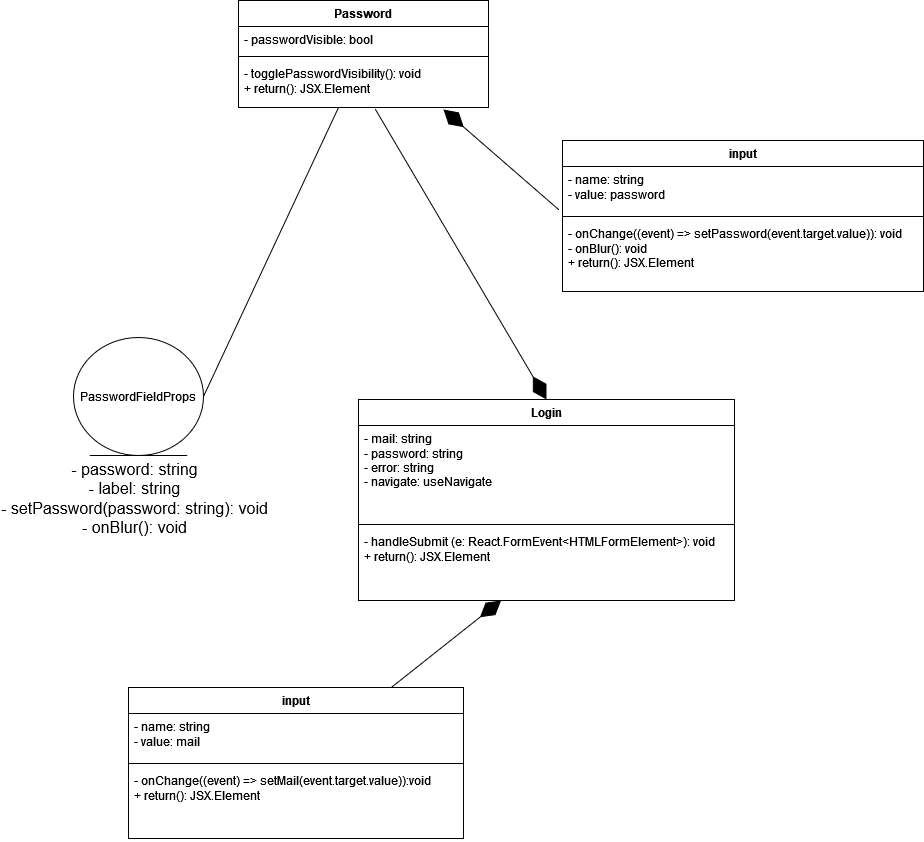
\includegraphics[width=1\textwidth, height=400pt]{documenti/imgUMLFrontend/LoginFEUML.drawio.png}
    \caption{UML Login}
    \label{fig:uml-login}
\end{figure}

Il componente \texttt{Login} è una funzione che prende una proprietà \texttt{onLogin} come parametro. Questo componente gestisce lo stato dell'email, della password e degli errori di login.\\
\custombold{Stato e Contesto}\\
\begin{itemize}
    \item \texttt{mail}: Memorizza l'email inserita dall'utente.
    \item \texttt{password}: Memorizza la password inserita dall'utente.
    \item \texttt{error}: Memorizza eventuali messaggi di errore.
\end{itemize}

\custombold{Funzione handleSubmit}\\
La funzione \texttt{handleSubmit} è chiamata quando l'utente invia il modulo di login:
\begin{enumerate}
    \item Previene il comportamento predefinito del modulo.
    \item Esegue un tentativo di login con l'API usando le credenziali fornite.
    \item Se il login ha successo (\texttt{LoginState.LOGGED\_IN}):
    \begin{itemize}
        \item Chiama la funzione \texttt{onLogin}.
        \item Memorizza il token nel \texttt{localStorage}.
        \item Naviga alla pagina principale.
    \end{itemize}
    \item Se l'utente deve registrarsi (\texttt{LoginState.MUST\_SIGN\_UP}):
    \begin{itemize}
        \item Naviga alla pagina di cambio password con l'email dell'utente.
    \end{itemize}
    \item In caso di fallimento, imposta un messaggio di errore.
\end{enumerate}
\custombold{Funzione handleBlur}\\
La funzione \texttt{handleBlur} azzera il messaggio di errore quando l'utente rimuove il focus dall'input.\\

\custombold{Rendering}\\
Il componente restituisce il markup JSX della pagina di login:
\begin{itemize}
    \item Un'intestazione "Login".
    \item Un modulo con:
    \begin{itemize}
        \item Un campo per l'email.
        \item Un componente \texttt{Password} per l'input della password, con una funzione \texttt{onBlur} per gestire il focus.
        \item Un messaggio di errore (se presente).
        \item Un pulsante di submit.
    \end{itemize}
    \item Un link per reimpostare la password in caso di password dimenticata.
\end{itemize}
\custombold{Interfaccia PasswordFieldProps}\\
Definisce le proprietà che il componente \texttt{Password} si aspetta di ricevere:
\begin{itemize}
    \item \textbf{password}: La stringa della password attuale.
    \item \textbf{setPassword}: Una funzione per aggiornare la password.
    \item \textbf{label}: Un'etichetta per il campo password.
    \item \textbf{onBlur}: Una funzione chiamata quando l'input perde il focus.
\end{itemize}

\custombold{Componente Password}\\
Il componente \texttt{Password} è una funzione di tipo \texttt{React.FC<PasswordFieldProps>} che utilizza le proprietà definite dall'interfaccia \texttt{PasswordFieldProps}.\\

\custombold{Stato}\\
\begin{itemize}
    \item \textbf{passwordVisible}: Uno stato booleano che determina se la password è visibile o meno. Inizialmente è impostato su \texttt{false}.
\end{itemize}

\custombold{Funzioni}\\
\begin{itemize}
    \item \textbf{togglePasswordVisibility}: Questa funzione inverte lo stato di \texttt{passwordVisible} quando viene chiamata, alternando la visibilità della password.
\end{itemize}
\custombold{Rendering}\\
Il componente restituisce il markup JSX del campo password:
\begin{itemize}
    \item Una \texttt{label} per il campo password, con il testo fornito dalla proprietà \texttt{label}.
    \item Un \texttt{div} contenitore per l'input della password e l'icona:
    \begin{itemize}
        \item Un \texttt{input} con le seguenti proprietà:
        \begin{itemize}
            \item \textbf{type}: Determina il tipo di input, che può essere \texttt{text} o \texttt{password} a seconda del valore di \texttt{passwordVisible}.
            \item \textbf{id} e \textbf{name}: Identificatori per il campo.
            \item \textbf{className}: Classe CSS per lo stile.
            \item \textbf{value}: Il valore della password, gestito dallo stato esterno.
            \item \textbf{onChange}: Una funzione chiamata quando il valore dell'input cambia, che aggiorna lo stato della password.
            \item \textbf{onBlur}: Una funzione chiamata quando l'input perde il focus, fornita dalle proprietà del componente.
            \item \textbf{required}: Specifica che il campo è obbligatorio.
        \end{itemize}
        \item Un'icona \texttt{FontAwesomeIcon} che cambia tra \texttt{faEye} e \texttt{faEyeSlash} a seconda dello stato di \texttt{passwordVisible}. Quando l'icona viene cliccata, chiama \texttt{togglePasswordVisibility} per alternare la visibilità della password.
    \end{itemize}
\end{itemize}

\subsubsection*{Cambio password}
\begin{figure}[H]
    \centering
    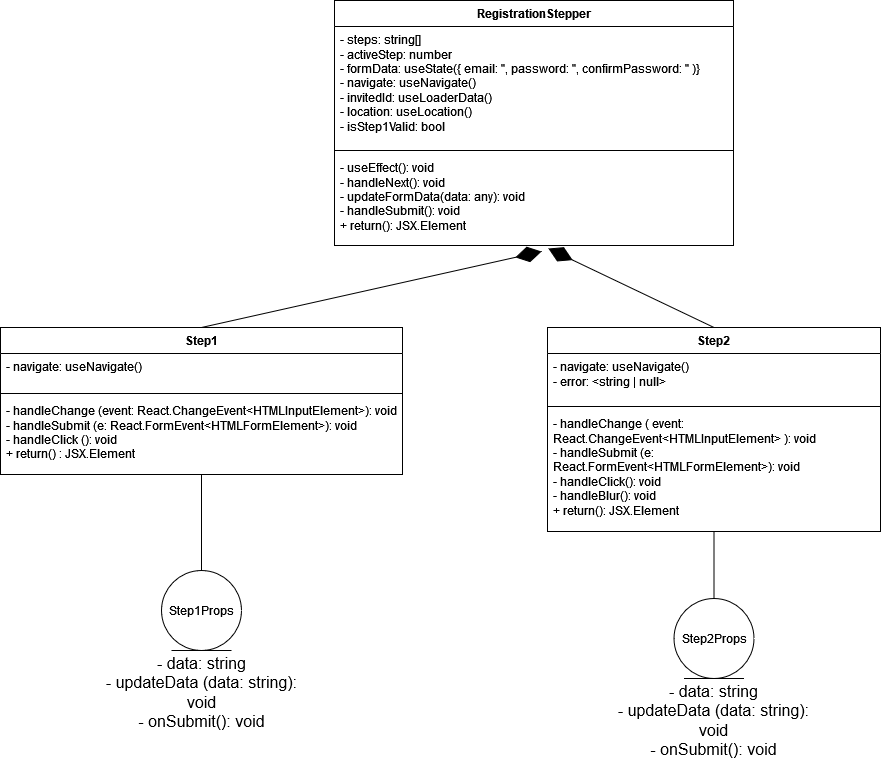
\includegraphics[width=1\textwidth, height=400pt]{documenti/imgUMLFrontend/RegistrationStepper.drawio.png}
    \caption{UML Cambio password}
    \label{fig:uml-cambio-password}
\end{figure}
Il componente \texttt{RegistrationStepper} è una funzione di tipo \texttt{React.FC} che gestisce il processo di registrazione a più fasi.
\custombold{Stato}\\
\begin{itemize}
    \item \texttt{activeStep}: Memorizza il passo attivo corrente dello stepper.
    \item \texttt{formData}: Memorizza i dati del modulo di registrazione, inclusi \texttt{email}, \texttt{password} e \texttt{confirmPassword}.
    \item \texttt{isStep1Valid}: Memorizza lo stato di validità del primo passo.
\end{itemize}
\custombold{Navigazione e Dati}\\
\begin{itemize}
    \item \texttt{navigate}: Hook per navigare tra le pagine.
    \item \texttt{inviteId}: Dati caricati utilizzando \texttt{useLoaderData}.
    \item \texttt{location}: Hook per ottenere la posizione corrente.
\end{itemize}
\custombold{Effetti}\\
\texttt{useEffect} viene utilizzato per validare i dati del primo passo:
\begin{itemize}
    \item Se \texttt{email} non è vuoto, \texttt{isStep1Valid} viene impostato su \texttt{true}.
    \item Altrimenti, \texttt{isStep1Valid} viene impostato su \texttt{false}.
\end{itemize}
\custombold{Funzioni}\\
\begin{itemize}
    \item \textbf{handleNext}: Avanza al passo successivo dello stepper se il passo attivo è inferiore alla lunghezza dei passi.
    \item \textbf{updateFormData}: Aggiorna i dati del modulo di registrazione.
    \item \textbf{handleSubmit}: Esegue la registrazione dell'utente, il login e l'accettazione dell'invito.
\end{itemize}
\custombold{Rendering}
Il componente restituisce il markup JSX dello stepper di registrazione:
\begin{itemize}
    \item Un \texttt{Box} contenente:
    \begin{itemize}
        \item Un'intestazione "Registrazione".
        \item Un componente \texttt{Stepper} con passi definiti.
        \item Un componente condizionale che rende \texttt{Step1} o \texttt{Step2} a seconda del passo attivo.
        \item Un \texttt{Box} per contenere i pulsanti di navigazione (non utilizzato in questo esempio).
    \end{itemize}
\end{itemize}
\custombold{Componente Step1}\\
Il componente \texttt{Step1} rappresenta il primo passo del processo di cambio password.
\custombold{Interfaccia Step1Props}\\
Definisce le proprietà che il componente \texttt{Step1} si aspetta di ricevere:
\begin{itemize}
    \item \texttt{data}: Un oggetto contenente l'email.
    \item \texttt{updateData}: Una funzione per aggiornare i dati del modulo.
    \item \texttt{onSubmit}: Una funzione chiamata quando il modulo viene inviato.
\end{itemize}
\custombold{Funzioni}\\
\begin{itemize}
    \item \textbf{handleChange}: Aggiorna l'email nei dati del modulo quando cambia il valore dell'input.
    \item \textbf{handleSubmit}: Previene il comportamento predefinito del modulo e chiama la funzione \texttt{onSubmit}.
    \item \textbf{handleClick}: Naviga alla pagina di login.
\end{itemize}
\custombold{Rendering}\\
Il componente restituisce il markup JSX del primo passo della modifica password:
\begin{itemize}
    \item Un \texttt{div} contenitore con una classe \texttt{container}.
    \item Un \texttt{form} con:
    \begin{itemize}
        \item Una \texttt{label} per l'email.
        \item Un \texttt{input} per inserire l'email.
        \item Un pulsante per inviare il modulo (Successivo).
        \item Un pulsante per navigare indietro (Indietro).
    \end{itemize}
\end{itemize}
\custombold{Componente Step2}\\
Il componente \texttt{Step2} rappresenta il secondo passo del processo di cambio password.
\custombold{Interfaccia Step2Props}\\
Definisce le proprietà che il componente \texttt{Step2} si aspetta di ricevere:
\begin{itemize}
    \item \texttt{data}: Un oggetto contenente \texttt{password} e \texttt{confirmPassword}.
    \item \texttt{updateData}: Una funzione per aggiornare i dati del modulo.
    \item \texttt{onSubmit}: Una funzione chiamata quando il modulo viene inviato.
\end{itemize}
\custombold{Funzioni}\\
\begin{itemize}
    \item \textbf{handleChange}: Aggiorna \texttt{password} e \texttt{confirmPassword} nei dati del modulo quando cambia il valore dell'input.
    \item \textbf{handleSubmit}: Previene il comportamento predefinito del modulo e controlla se \texttt{password} e \texttt{confirmPassword} corrispondono. Se non corrispondono, imposta un messaggio di errore. Altrimenti, chiama la funzione \texttt{onSubmit}.
    \item \textbf{handleClick}: Naviga al primo passo della registrazione.
    \item \textbf{handleBlur}: Azzera il messaggio di errore quando l'input perde il focus.
\end{itemize}
\custombold{Rendering}\\
Il componente restituisce il markup JSX del secondo passo della modifica password:
\begin{itemize}
    \item Un \texttt{div} contenitore.
    \item Un \texttt{form} con:
    \begin{itemize}
        \item Due componenti \texttt{Password} per inserire \texttt{password} e \texttt{confirmPassword}.
        \item Un messaggio di errore (se presente).
        \item Un pulsante per inviare il modulo (Invia).
        \item Un pulsante per navigare indietro (Indietro).
    \end{itemize}
\end{itemize}

\subsection{Table}
\begin{figure}[H]
    \centering
    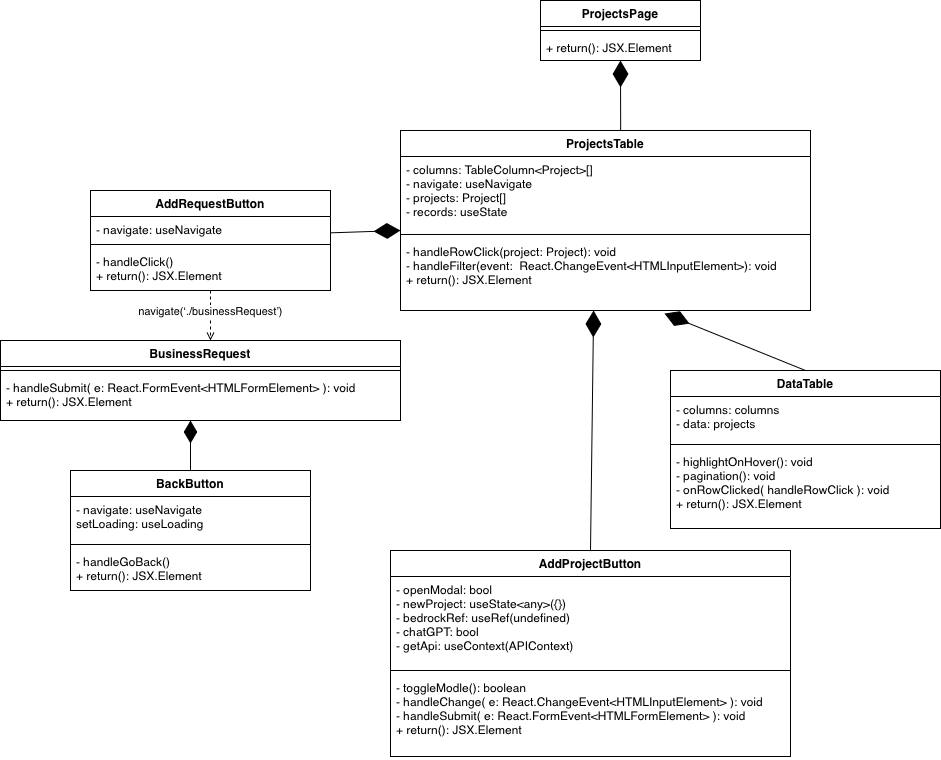
\includegraphics[width=1\textwidth, height=400pt]{documenti/imgUMLFrontend/Project.jpg}
    \caption{UML Progetto}
    \label{fig:uml-project}
\end{figure}

Il componente \texttt{ProjectsTable} è un componente React che visualizza una tabella di progetti utilizzando il pacchetto \texttt{react-data-table-component}. Il componente permette all'utente di filtrare i progetti tramite un campo di ricerca e di navigare ai dettagli di un progetto selezionato.
Il componente Table corrisponde alla parte principale della web app. Qua si possono vedere tutti i progetti, in più solo il Project Manager può creare nuovi progetti e solo il cliente potrà proporre i requisiti di business.

\subsubsection*{Stato Interno}
\begin{itemize}
    \item \texttt{records}: Stato che memorizza i progetti filtrati visualizzati nella tabella.
\end{itemize}

\subsubsection*{Contesto}
\begin{itemize}
    \item \texttt{projects}: Dati dei progetti caricati tramite \texttt{useLoaderData}.
    \item \texttt{isLoading}: Stato del caricamento gestito dal contesto \texttt{LoadingContext}.
\end{itemize}

\subsection*{Funzione \texttt{handleFilter}}

La funzione \texttt{handleFilter} aggiorna lo stato \texttt{records} in base al testo inserito dall'utente nel campo di ricerca.


\subsubsection*{Effetti}

\begin{itemize}
    \item \texttt{useEffect}: Gestisce lo stato di caricamento in base allo stato della navigazione.
\end{itemize}

\subsubsection*{Rendering}

Il componente restituisce il markup JSX della tabella dei progetti:

\begin{itemize}
    \item \texttt{AddProjectButton}: Pulsante per aggiungere un nuovo progetto.
    \item \texttt{AddRequestButton}: Pulsante per aggiungere una nuova richiesta.
    \item \texttt{input}: Campo di ricerca per filtrare i progetti.
    \item \texttt{ClipLoader}: Spinner di caricamento visualizzato durante l'operazione di caricamento.
    \item \texttt{DataTable}: Componente della tabella che visualizza i progetti.
\end{itemize}

\subsubsection*{Colonne della Tabella}

\begin{itemize}
    \item \texttt{Titolo}: Nome del progetto.
    \item \texttt{Cliente}: Nome del cliente associato al progetto.
    \item \texttt{Data di Inizio}: Data di inizio del progetto.
    \item \texttt{Progress}: Stato di avanzamento del progetto visualizzato come barra di progresso.
\end{itemize}

\subsubsection*{Gestione del Click sulla Riga}

Quando una riga della tabella viene cliccata, l'utente viene navigato alla pagina dei dettagli del progetto.

\subsection*{AddProjectButton}

Il componente \texttt{AddProjectButton} è un componente React che permette all'utente di creare un nuovo progetto tramite un modal. Utilizza i componenti di \texttt{mdb-react-ui-kit} per la costruzione del modal e dei suoi elementi interattivi.

\subsubsection*{Stato Interno}
\begin{itemize}
    \item \texttt{openModal}: Booleano che gestisce l'apertura e la chiusura del modal.
    \item \texttt{newProject}: Oggetto che contiene i dati del nuovo progetto da creare.
    \item \texttt{bedrockRef}: Riferimento al componente radio per determinare l'AI scelta.
    \item \texttt{chatGPT}: Booleano che gestisce lo stato della scelta dell'AI.
\end{itemize}

\subsubsection*{Funzione \texttt{toggleModal}}

La funzione \texttt{toggleModal} gestisce l'apertura e la chiusura del modal.

\subsubsection*{Funzione \texttt{handleChange}}

La funzione \texttt{handleChange} aggiorna lo stato \texttt{newProject} in base ai dati inseriti dall'utente nei campi di input.

\subsubsection*{Funzione \texttt{handleSubmit}}

La funzione \texttt{handleSubmit} gestisce l'invio del form e l'aggiunta del nuovo progetto tramite l'API.

\subsubsection*{Rendering}

Il componente restituisce il markup JSX del pulsante e del modal per la creazione del nuovo progetto:

\begin{itemize}
    \item \texttt{button}: Pulsante per aprire il modal.
    \item \texttt{MDBModal}: Modal che contiene il form per la creazione del progetto.
    \item \texttt{MDBModalDialog}: Dialog del modal centrato.
    \item \texttt{MDBModalContent}: Contenuto del modal.
    \item \texttt{MDBModalHeader}: Header del modal con il titolo e il pulsante per chiudere.
    \item \texttt{MDBModalBody}: Corpo del modal che contiene il form.
    \item \texttt{MDBModalFooter}: Footer del modal con i pulsanti per inviare o annullare.
    \item \texttt{MDBInput}, \texttt{MDBRadio}: Componenti di input e radio per il form.
\end{itemize}

\subsubsection*{Componenti del Form}

\begin{itemize}
    \item \texttt{input} per il titolo del progetto.
    \item \texttt{textarea} per la descrizione del progetto.
    \item \texttt{MDBRadio} per la selezione del tipo di AI (ChatGPT o Bedrock).
\end{itemize}

\subsection*{AddRequestButton-BusinessRequest}
 Il componente  \texttt{AddRequestButton} fornisce un pulsante per navigare alla pagina di richiesta business, mentre \texttt{BusinessRequest} fornisce un form per inviare i requisiti di business ad un'API.


\subsubsection*{Descrizione}

Il componente \texttt{AddRequestButton} è un semplice pulsante che, quando cliccato, reindirizza l'utente alla pagina \texttt{/businessRequest} utilizzando il hook \texttt{useNavigate} di React Router.


\subsubsection*{Proprietà}
Il componente \texttt{AddRequestButton} non accetta proprietà.

\subsubsection*{Stato Interno}
Il componente \texttt{AddRequestButton} non mantiene stato interno.


\subsubsection*{Funzione \texttt{handleClick}}
Questa funzione viene chiamata al click del pulsante e naviga l'utente alla pagina \texttt{/businessRequest}.

\subsubsection*{\texttt{BusinessRequest}}

\subsubsection*{Descrizione}

Il componente \texttt{BusinessRequest} fornisce un form che permette all'utente di inserire e inviare requisiti di business tramite un'API. Utilizza il hook \texttt{useRef} per ottenere il valore del campo textarea e inviarlo tramite la funzione \texttt{handleSubmit}.

\subsubsection*{Proprietà}
Il componente \texttt{BusinessRequest} non accetta proprietà.

\subsubsection*{Stato Interno}
Il componente \texttt{BusinessRequest} non mantiene stato interno.


\subsubsection*{Funzione \texttt{handleSubmit}}
Questa funzione viene chiamata al submit del form, previene il comportamento predefinito del submit, ottiene il valore della textarea tramite il riferimento \texttt{input}, e invia questo valore all'API tramite la funzione \texttt{api.sendBusinessRequirementsToAI}.

\subsubsection*{Rendering dei Componenti}

\subsubsection*{Componente \texttt{AddRequestButton}}

Il componente \texttt{AddRequestButton} restituisce il markup JSX di un pulsante che, quando cliccato, reindirizza l'utente alla pagina \texttt{/businessRequest}.

\subsubsection*{Componente \texttt{BusinessRequest}}

Il componente \texttt{BusinessRequest} restituisce il markup JSX di un form con una textarea per inserire i requisiti di business e un pulsante per inviare il form. Comprende anche un header per il titolo "Requisiti di Business".


\subsection{EpicStory}
\begin{figure}[H]
    \centering
    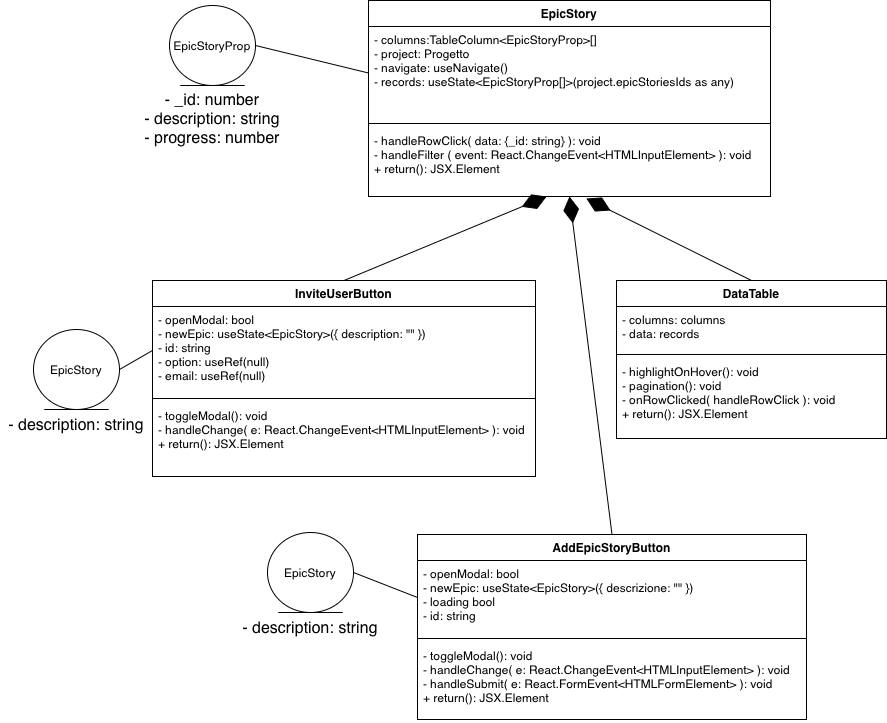
\includegraphics[width=1\textwidth, height=400pt]{documenti/imgUMLFrontend/Epic.jpg}
    \caption{UML Epic Story}
    \label{fig:uml-epicStory}
\end{figure}
Il componente \texttt{EpicStory} visualizza le epic story di un progetto, mentre il componente \texttt{EpicDetails} visualizza i dettagli di una specifica epic story.


\subsubsection*{Descrizione}

Il componente \texttt{EpicStory} visualizza le epic story di un progetto. Consente all'utente di filtrare le epic story per nome e di cliccare su una epic story per visualizzare i dettagli.

\subsubsection*{Stato Interno}
Il componente \texttt{EpicStory} mantiene uno stato interno per gestire le epic story visualizzate.


\subsubsection*{Funzione \texttt{handleRowClick}}
Questa funzione viene chiamata quando l'utente clicca su una riga della tabella delle epic story. Naviga l'utente alla pagina dei dettagli della epic story corrispondente.

\subsubsection*{Funzione \texttt{handleFilter}}
Questa funzione viene chiamata quando l'utente digita nel campo di ricerca. Filtra le epic story in base al nome.

\subsubsection*{Descrizione}

Il componente \texttt{EpicDetails} visualizza i dettagli di una specifica epic story. In questo caso, visualizza le user story associate alla epic story selezionata.

\subsubsection*{Stato Interno}
Il componente \texttt{EpicDetails} mantiene uno stato interno per gestire i dettagli della epic story e le user story associate.

\subsubsection*{Funzioni Principali}

Il componente \texttt{EpicDetails} non contiene funzioni principali oltre all'effetto di caricamento dei dati.

\subsection*{InviteUserButton}
Il componente \textbf{InviteUserButton} è responsabile della visualizzazione di un pulsante che apre un modale per invitare un utente a un progetto.

\subsubsection*{Stato Interno}
\begin{itemize}
    \item \textbf{openModal}: booleano che indica se il modale è aperto o chiuso.
    \item \textbf{newEpic}: oggetto che rappresenta la nuova epic story inserita dall'project manager.
\end{itemize}

\subsubsection*{Funzioni Principali}
\begin{itemize}
    \item \textbf{toggleModal}: funzione che cambia lo stato di \textit{openModal}, aprendo o chiudendo il modale.
    \item \textbf{handleChange}: funzione che gestisce il cambiamento di valore degli input dell'utente.
    \item \textbf{handleSubmit}: funzione che gestisce l'invio del form per l'invito dell'utente al progetto.
\end{itemize}

\subsubsection*{Rendering}
Il componente \textbf{InviteUserButton} rende un pulsante che, quando cliccato, apre un modale. Il modale contiene un campo di input per l'email dell'utente da invitare e un menu a tendina per selezionare il ruolo dell'utente (cliente o sviluppatore). In fondo al modale, ci sono pulsanti per confermare o annullare l'operazione di invito.

\subsection*{AddEpicStoryButton}

\subsubsection*{Descrizione}
Il componente \textbf{AddEpicStoryButton} è responsabile della visualizzazione di un pulsante che apre un modale per consentire all'project manager di aggiungere una nuova epic story.

\subsubsection*{Stato Interno}
\begin{itemize}
    \item \textbf{openModal}: booleano che indica se il modale è aperto o chiuso.
    \item \textbf{newEpic}: oggetto che rappresenta la nuova epic story inserita dall'utente.
    \item \textbf{loading}: booleano che indica se è in corso un'operazione di caricamento.
\end{itemize}

\subsubsection*{Funzioni Principali}
\begin{itemize}
    \item \textbf{toggleModal}: funzione che cambia lo stato di \textit{openModal}, aprendo o chiudendo il modale.
    \item \textbf{handleChange}: funzione che gestisce il cambiamento di valore dell'input della descrizione della nuova epic story.
    \item \textbf{handleSubmit}: funzione che gestisce l'invio del form per l'aggiunta della nuova epic story al progetto.
\end{itemize}

\subsubsection*{Rendering}
Il componente \textbf{AddEpicStoryButton} rende un pulsante che, quando cliccato, apre un modale. Il modale contiene un campo di input per la descrizione della nuova epic story. In fondo al modale, ci sono pulsanti per confermare o annullare l'aggiunta della epic story.


\subsection{UserStory}
\begin{figure}[H]
    \centering
    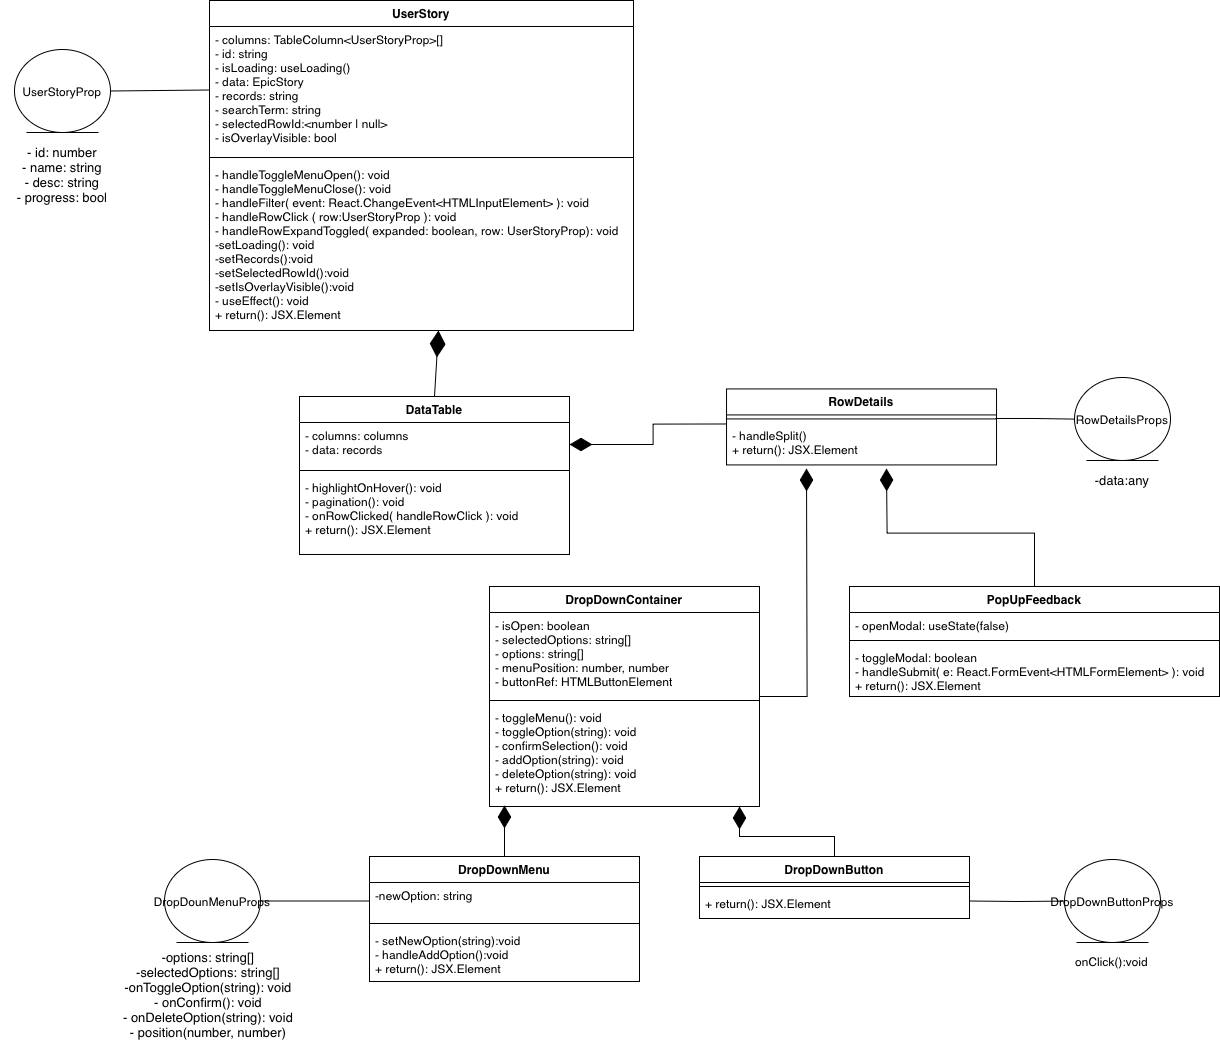
\includegraphics[width=1\textwidth, height=400pt]{documenti/imgUMLFrontend/User.jpg}
    \caption{UML User Story}
    \label{fig:uml-userStory}
\end{figure}
Il componente \textbf{UserStory} è responsabile della visualizzazione delle storie degli utenti all'interno di una tabella, con possibilità di ricerca, selezione e visualizzazione dei dettagli di ogni user story.

\subsubsection*{Stato Interno}
\begin{itemize}
    \item \textbf{records}: array di oggetti che rappresentano le storie degli utenti.
    \item \textbf{searchTerm}: stringa che rappresenta il termine di ricerca inserito dall'utente.
    \item \textbf{selectedRowId}: identificatore della riga selezionata.
    \item \textbf{isOverlayVisible}: booleano che indica se l'overlay per il menu è visibile o meno.
\end{itemize}

\subsubsection*{Funzioni Principali}
\begin{itemize}
    \item \textbf{handleFilter}: funzione per filtrare le storie degli utenti in base al termine di ricerca inserito dall'utente.
    \item \textbf{handleRowClick}: funzione per gestire il click su una riga della tabella, selezionandola o deselezionandola.
    \item \textbf{handleRowExpandToggled}: funzione per gestire l'espansione o la chiusura di una riga della tabella.
    \item \textbf{handleToggleMenuOpen, handleToggleMenuClose}: funzioni per aprire e chiudere l'overlay del menu.
\end{itemize}

\subsubsection*{Rendering}
Il componente \textbf{UserStory} rende una tabella contenente le storie degli utenti. Ogni riga della tabella mostra il tag, il titolo e lo stato di completamento della user story. È presente un campo di ricerca per filtrare le storie degli utenti. È possibile selezionare una riga della tabella per visualizzare i dettagli della user story.

\subsection*{RowDetails}
Il componente \textbf{RowDetails} è responsabile della visualizzazione dei dettagli di una riga della tabella delle storie degli utenti.

\subsubsection*{Proprietà}

\begin{itemize}
    \item \textbf{data}: oggetto che contiene i dati della riga della tabella.
\end{itemize}

\subsubsection*{Funzioni Principali}
\begin{itemize}
    \item \textbf{handleSplit}: funzione per gestire la divisione di una user story in due user story, mandando la richiesta all'intelligenza artificiale.
\end{itemize}

\subsubsection*{Rendering}
Il componente \textbf{RowDetails} rende i dettagli di una riga della tabella delle storie degli utenti, inclusa la descrizione della user story e i componenti \textit{DropdownContainer} e \textit{PopupFeedback}. Inoltre, include un pulsante per eseguire l'azione di divisione della riga.

\subsection*{PopUpFeedback}
Il componente PopupFeedback è stato implementato utilizzando React ed è composto dai seguenti elementi:

\subsubsection*{Stato}
Il componente utilizza uno stato locale per gestire l'apertura e la chiusura della finestra modale.

\subsubsection*{Funzionalità}
Il componente fornisce le seguenti funzionalità:
\begin{itemize}
    \item Mostra un pulsante "Feedback".
    \item Quando il pulsante "Feedback" viene cliccato, viene visualizzata una finestra modale.
    \item La finestra modale contiene un modulo per inserire il feedback.
    \item Gli utenti possono inserire il loro feedback nel modulo.
    \item Gli utenti possono inviare il feedback all'intelligenza artificiale tramite il pulsante "Invia".
    \item Gli utenti possono annullare l'operazione e chiudere la finestra modale tramite il pulsante "Annulla".
\end{itemize}

\subsection*{DropDownContainer}
Il componente \texttt{DropdownContainer} gestisce il menu a discesa per l'assegnazione degli sviluppatori alla user story e le azioni associate ai pulsanti.
Questo componente offre un'interfaccia intuitiva e interattiva per la selezione delle opzioni tramite un menu a discesa.
\subsubsection*{Funzionalità Principali}

\begin{enumerate}
    \item \textbf{Gestione dello Stato}:
    \begin{itemize}
        \item Utilizza lo stato per gestire l'apertura e la chiusura del menu a discesa (\texttt{isOpen}).
        \item Mantiene lo stato delle opzioni selezionate (\texttt{selectedOptions}).
        \item Memorizza la lista delle opzioni disponibili (\texttt{options}).
        \item Conserva la posizione del menu a discesa rispetto al pulsante associato (\texttt{menuPosition}).
    \end{itemize}
    
    \item \textbf{Interazione Utente}:
    \begin{itemize}
        \item Fornisce un pulsante per aprire e chiudere il menu a discesa.
        \item Gestisce l'apertura e la chiusura del menu a discesa quando il pulsante viene cliccato.
        \item Passa la posizione calcolata del menu a discesa al componente \texttt{DropdownMenu} tramite le proprietà.
    \end{itemize}
    
    \item \textbf{Gestione delle Opzioni}:
    \begin{itemize}
        \item Consente all'utente di selezionare o deselezionare le opzioni nel menu a discesa, ovvero gli sviluppatori.
        \item Permette all'utente di confermare le selezioni fatte.
        \item Fornisce funzionalità per aggiungere nuovi sviluppatori alla lista e per eliminarne.
    \end{itemize}
    
    \item \textbf{Utilizzo di useRef}:
    \begin{itemize}
        \item Utilizza \texttt{useRef} per ottenere un riferimento al pulsante associato al menu a discesa.
    \end{itemize}
    
    \item \textbf{Utilizzo di ReactDOM.createPortal}:
    \begin{itemize}
        \item Utilizza \texttt{ReactDOM.createPortal} per montare il componente \texttt{DropdownMenu} nel nodo del DOM del \texttt{<body>}, garantendo la corretta sovrapposizione del menu agli altri elementi della pagina.
    \end{itemize}
\end{enumerate}

\subsubsection*{Componenti Associati}

\begin{itemize}
    \item \texttt{DropdownButton}: Rappresenta il pulsante per aprire il menu a discesa.
    \item \texttt{DropdownMenu}: Rappresenta il menu a discesa che mostra le opzioni disponibili e consente all'utente di selezionarle.
\end{itemize}

\subsection*{DropDownButton}
Il componente \texttt{DropdownButton} rappresenta il pulsante per aprire il menu a discesa.

\subsubsection*{Caratteristiche Principali}

\begin{enumerate}
    \item \textbf{Utilizzo di forwardRef}:
    \begin{itemize}
        \item Utilizza \texttt{forwardRef} per ottenere un riferimento al pulsante e renderlo disponibile al componente genitore.
        \item Questo consente al componente genitore di interagire direttamente con il pulsante, ad esempio per impostare il focus o accedere ad altre proprietà.
    \end{itemize}
    
    \item \textbf{Proprietà}:
    \begin{itemize}
        \item \texttt{onClick}: Una funzione da eseguire quando il pulsante viene cliccato. In genere, questa funzione apre il menu a discesa.
    \end{itemize}
\end{enumerate}

\subsection*{DropDownMenu}
Il componente \texttt{DropdownMenu} rappresenta il menu a discesa che visualizza gli sviluppatori selezionabili.

\subsubsection*{Caratteristiche Principali}

\begin{enumerate}
    \item \textbf{Proprietà}:
    \begin{itemize}
        \item \texttt{options}: Un array di stringhe rappresentanti le opzioni disponibili nel menu.
        \item \texttt{selectedOptions}: Un array di stringhe che rappresenta le opzioni attualmente selezionate.
        \item \texttt{onToggleOption}: Una funzione chiamata quando una opzione viene selezionata o deselezionata.
        \item \texttt{onConfirm}: Una funzione chiamata quando l'utente conferma le selezioni nel menu.
        \item \texttt{onAddOption}: Una funzione chiamata quando una nuova opzione viene aggiunta al menu.
        \item \texttt{onDeleteOption}: Una funzione chiamata quando un'opzione esistente viene eliminata dal menu.
        \item \texttt{position}: Un oggetto che contiene le coordinate della posizione del menu nella pagina.
    \end{itemize}
    
    \item \textbf{Gestione Aggiunta di Opzioni}:
    \begin{itemize}
        \item Il menu fornisce un'interfaccia per aggiungere nuove opzioni attraverso un campo di input e un pulsante di aggiunta.
    \end{itemize}
\end{enumerate}

\subsection{Barra di navigazione}
\begin{figure}[H]
    \centering
    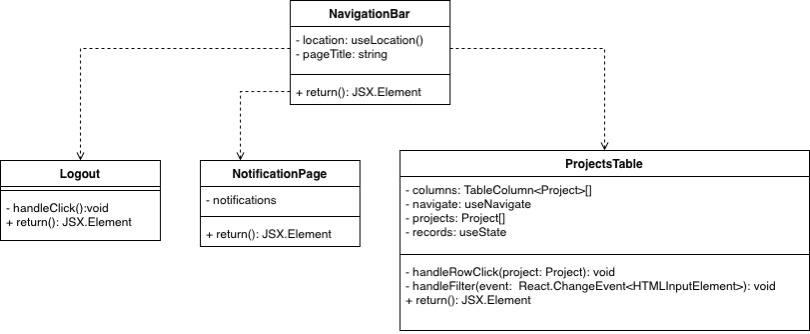
\includegraphics[width=\textwidth]{documenti/imgUMLFrontend/NavBar.jpg}
    \caption{UML NavigationBar}
    \label{fig:uml-navigatio}
\end{figure}

Il componente \texttt{NavigationBar} rappresenta una barra di navigazione che mostra un titolo di pagina basato sul percorso corrente e fornisce collegamenti per la navigazione tra diverse pagine.

\subsubsection*{Caratteristiche Principali}

\begin{enumerate}
    \item \textbf{Proprietà}:
    \begin{itemize}
        \item \texttt{routeTitles}: Un oggetto di mapping tra i percorsi e i relativi titoli di pagina.
        \item \texttt{location}: Un hook di React Router (\texttt{useLocation}) che fornisce informazioni sul percorso corrente.
    \end{itemize}

    \item \textbf{Elementi del DOM}:
    \begin{itemize}
        \item \texttt{<nav>}: Elemento principale della barra di navigazione.
        \item \texttt{<div className="left">}: Contenitore per il titolo della pagina.
        \item \texttt{<div className="right">}: Contenitore per i link di navigazione e il pulsante di logout.
        \item \texttt{<h1>}: Titolo della pagina, dinamicamente aggiornato in base al percorso corrente.
        \item \texttt{<Link>}: Componenti di React Router per la navigazione tra pagine.
        \item \texttt{<a>}: Elemento per il componente di logout.
    \end{itemize}
    
    \item \textbf{Funzionalità}:
    \begin{itemize}
        \item Determina il titolo della pagina corrente in base al percorso utilizzando l'oggetto \texttt{routeTitles}.
        \item Fornisce collegamenti di navigazione alle pagine "Progetti" e "Notifiche".
        \item Include un componente per il logout.
    \end{itemize}
\end{enumerate}

\subsection*{Logout}
Il componente \textbf{Logout} è responsabile della gestione del logout dell'utente. Quando l'utente clicca sul pulsante di logout, il token di autenticazione viene rimosso dal \texttt{localStorage} del browser e l'utente viene disconnesso.

\subsubsection*{Funzioni Principali}
\begin{itemize}
    \item \textbf{handleClick}: funzione che viene chiamata quando l'utente clicca sul pulsante di logout. Questa funzione rimuove il token di autenticazione dal \texttt{localStorage}.
\end{itemize}

\subsubsection*{Rendering}
Il componente \textbf{Logout} rende un pulsante con un'icona di logout. Quando l'utente clicca sul pulsante, viene eseguita la funzione \texttt{handleClick}.

\subsubsection*{Componenti Utilizzati}
\begin{itemize}
    \item \textbf{FontAwesomeIcon}:
    \begin{itemize}
        \item \texttt{@fortawesome/react-fontawesome}: Libreria per l'uso delle icone FontAwesome in React.
        \item \texttt{@fortawesome/free-solid-svg-icons}: Pacchetto di icone gratuite di FontAwesome.
        \item \texttt{faSignOutAlt}: Icona di uscita utilizzata nel pulsante di logout.
    \end{itemize}
\end{itemize}


\subsection{Notifiche}
\begin{figure}[H]
    \centering
    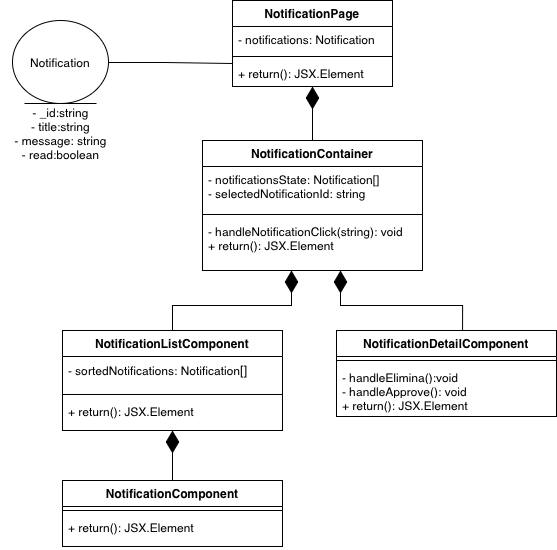
\includegraphics[width=1\textwidth, height=400pt]{documenti/imgUMLFrontend/Notifica.jpg}
    \caption{UML Notifiche}
    \label{fig:uml-notifiche}
\end{figure}

Il componente \textbf{NotificationPage} è responsabile della visualizzazione delle notifiche e dei dettagli delle notifiche per un utente. Utilizza diversi componenti presentazionali e container per gestire lo stato e la logica delle notifiche.

\subsubsection*{Stato Interno}
\begin{itemize}
    \item \textbf{notificationsState}: array di notifiche mantenuto dallo stato del componente.
    \item \textbf{selectedNotificationId}: ID della notifica selezionata, inizialmente nullo.
\end{itemize}

\subsubsection*{Funzioni Principali}
\begin{itemize}
    \item \textbf{handleNotificationClick}: funzione che gestisce il click su una notifica. Marca la notifica come letta e aggiorna lo stato.
    \item \textbf{handleApprove}: funzione che approva una notifica e crea un nuovo progetto basato sulla notifica.
\end{itemize}

\subsubsection*{Rendering}
Il componente \textbf{NotificationPage} rende un container con una lista di notifiche e i dettagli della notifica selezionata. La lista è ordinata in modo da mostrare prima le notifiche non lette.

\subsubsection*{Componenti Utilizzati}
\begin{itemize}
    \item \textbf{NotificationComponent}:
    \begin{itemize}
        \item Mostra una singola notifica con il titolo, il messaggio e un indicatore di lettura.
    \end{itemize}
    \item \textbf{NotificationListComponent}:
    \begin{itemize}
        \item Mostra una lista di notifiche ordinate per stato di lettura.
    \end{itemize}
    \item \textbf{NotificationDetailComponent}:
    \begin{itemize}
        \item Mostra i dettagli della notifica selezionata con pulsanti per approvare o eliminare.
    \end{itemize}
    \item \textbf{NotificationContainer}:
    \begin{itemize}
        \item Gestisce lo stato delle notifiche e la logica per la selezione e la lettura delle notifiche.
    \end{itemize}
    \item \textbf{api}:
    \begin{itemize}
        \item Funzioni per interagire con l'API del backend, come \texttt{readNotification} e \texttt{addProject}.
    \end{itemize}
    \item \textbf{createEpicStoriesFromBR}:
    \begin{itemize}
        \item Funzione che utilizza l'IA per creare epic stories da un business requirement.
    \end{itemize}
\end{itemize}



\subsection{Architettura Backend}
Per il backend del servizio è stata selezionata l'adozione del modello di Serverless Architecture. Questo paradigma di cloud computing consente lo sviluppo e la gestione delle applicazioni senza la necessità di amministrare direttamente i server fisici. Tale modello garantisce una scalabilità elevata, un'alta disponibilità, e costi contenuti, eliminando la preoccupazione relativa all'infrastruttura sottostante. Grazie a questa architettura, sarà infatti possibile effettuare una scalabilità dinamica, adattando le risorse disponibili alle specifiche esigenze del servizio in tempo reale, sia incrementandole che riducendole, a seconda delle necessità operative.
 \begin{figure}[H]
      \centering
      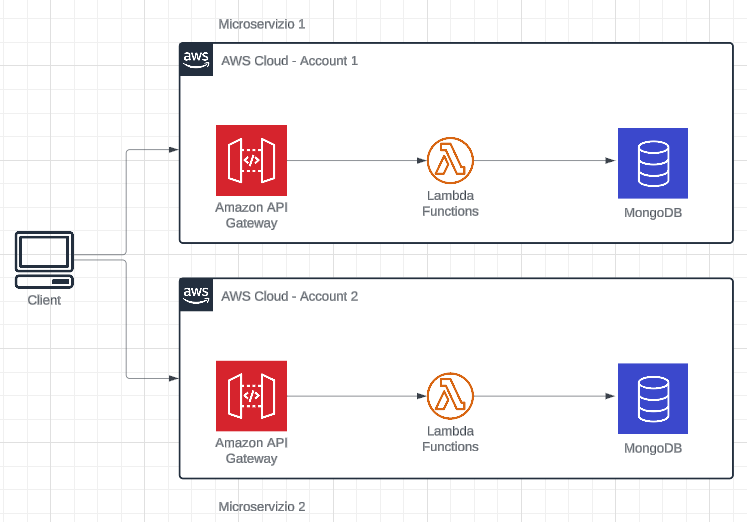
\includegraphics{documenti/grafici/schema serverless architecture pattern.png}
      \caption{Schema architettura serverless}
      \label{fig: archser}
    \end{figure}
\subsubsection{Diagramma delle classi}
 \begin{figure}[H]
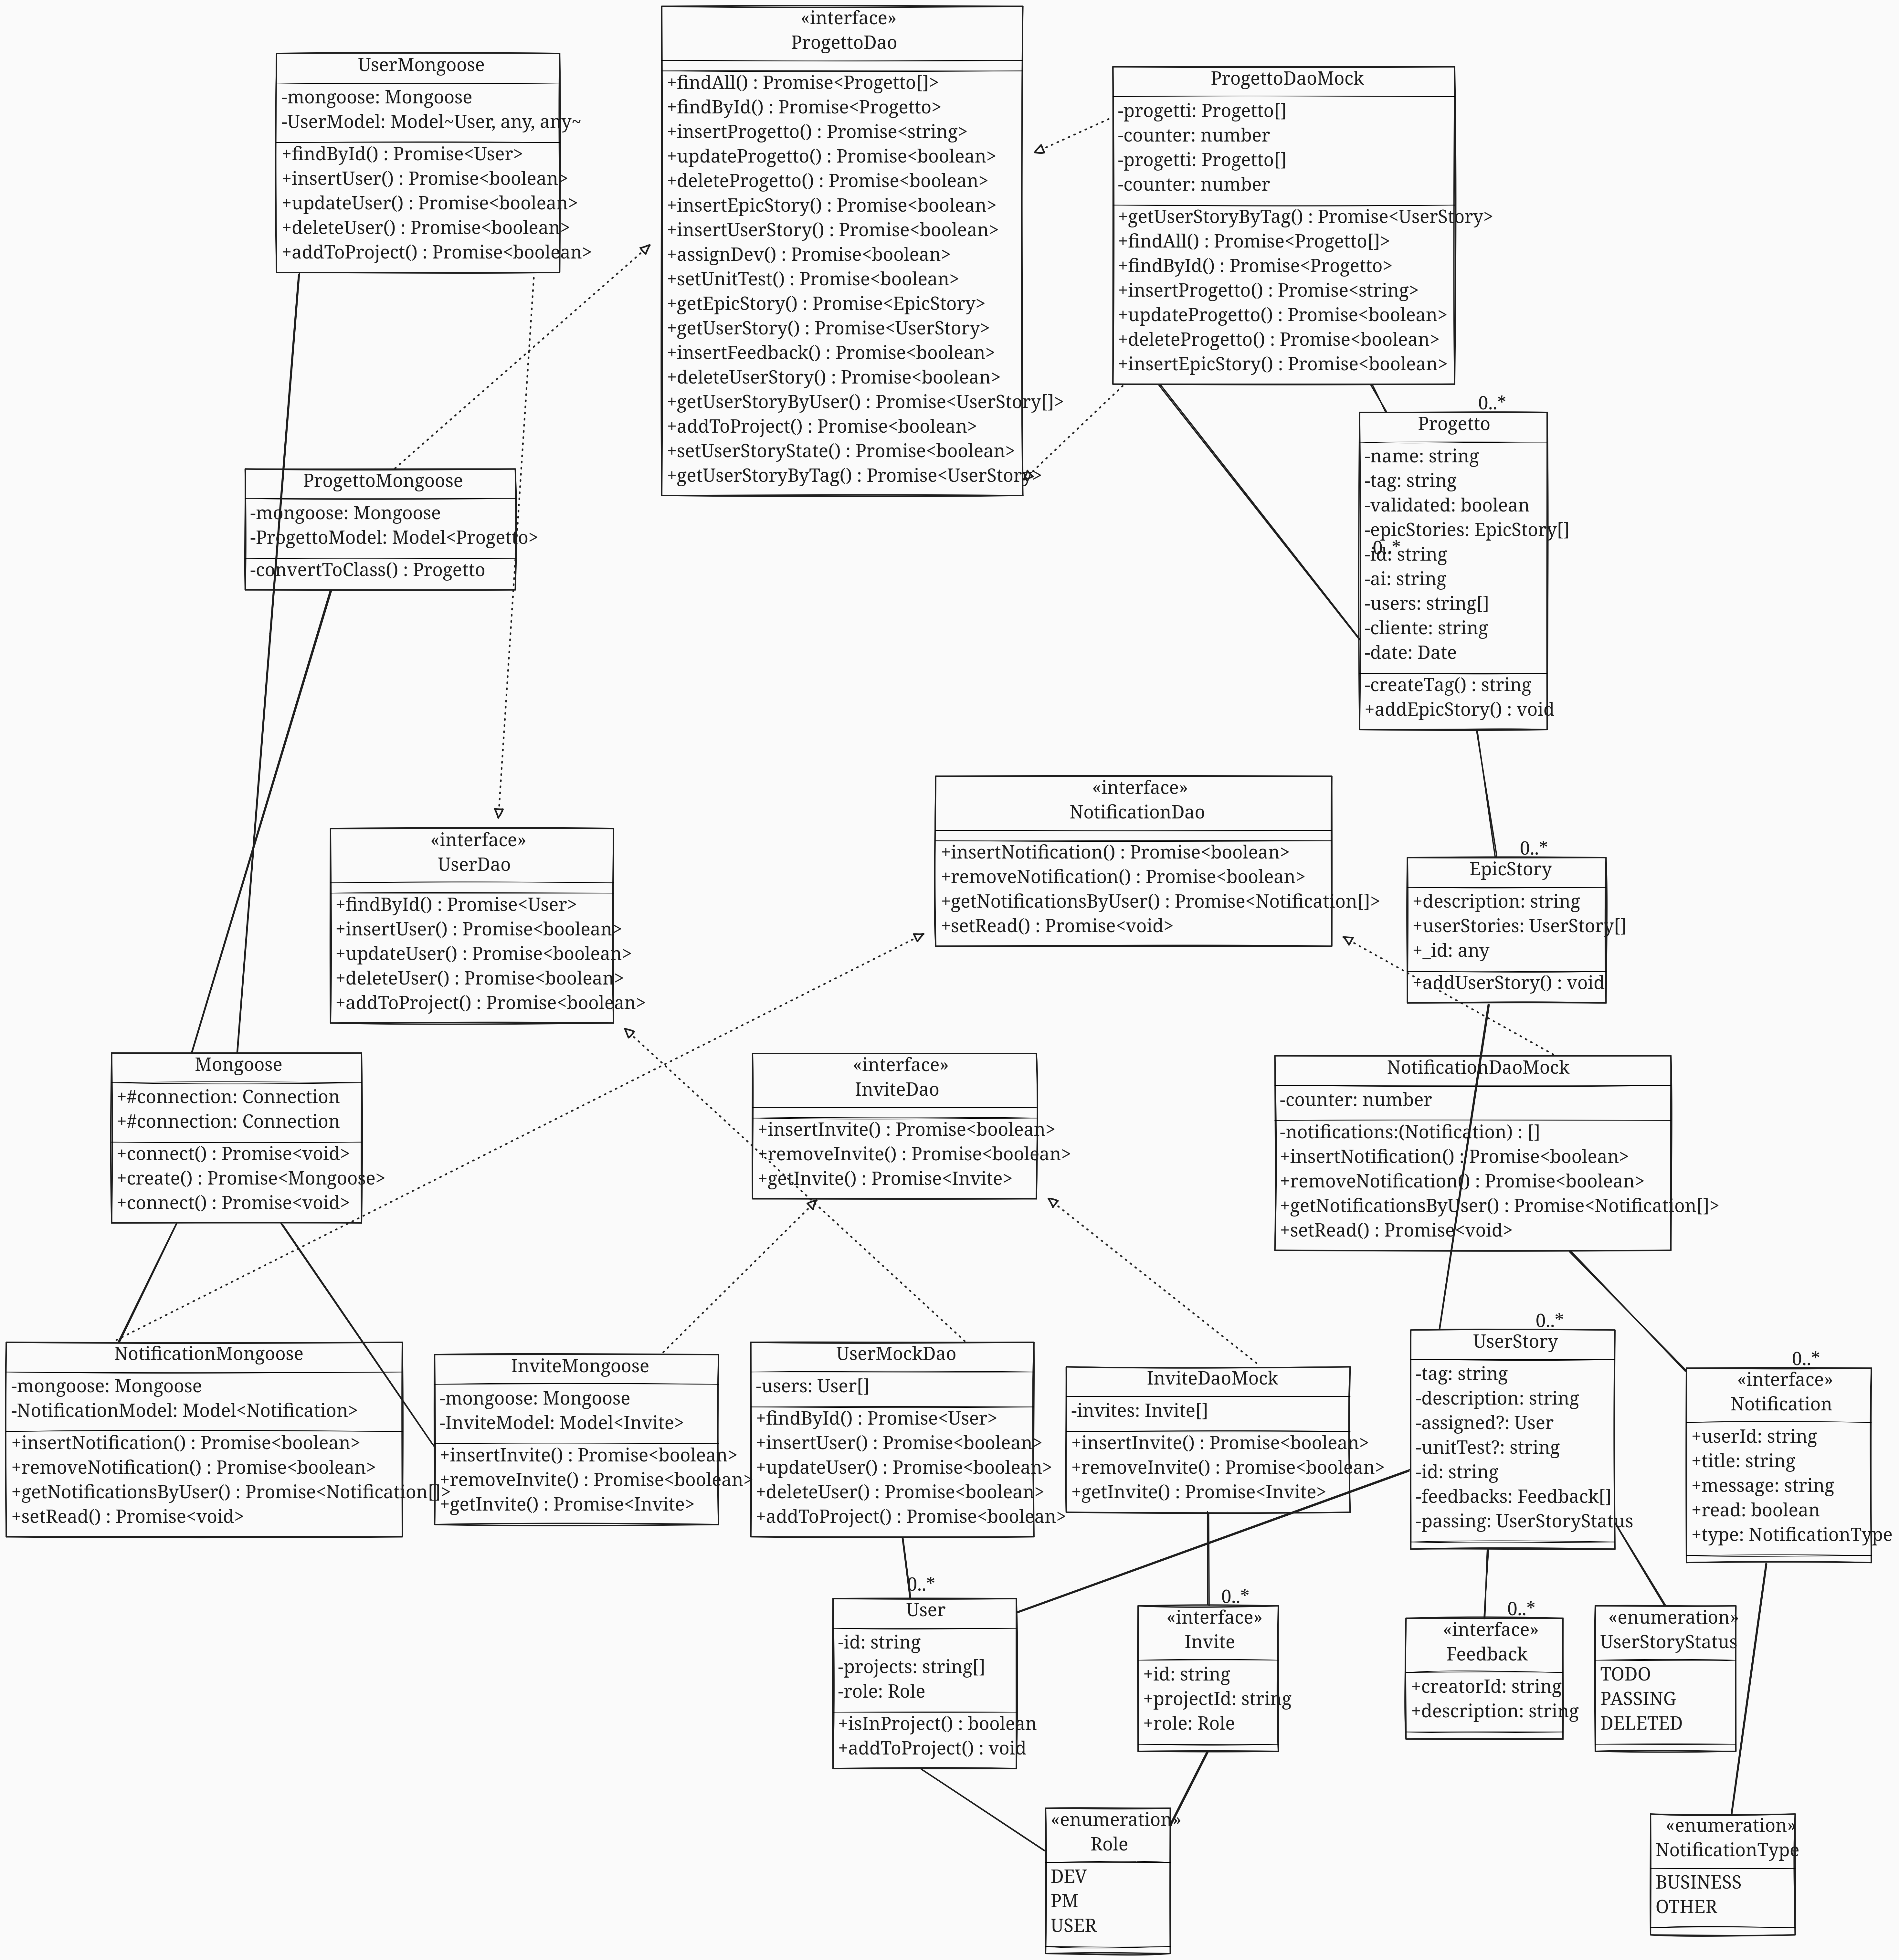
\includegraphics[width=1.1\textwidth]{documenti/imgUML/uml-backend.png}
\caption{Schema delle classi Backend}
\label{fig: archser}
\end{figure}
\begin{itemize}
\item \textbf{Classe: \textit{Mongoose}}
\begin{itemize}
\item Attributi
\begin{itemize}
\item \custombold{connection: Connection}: La connessione al database.
\end{itemize}
\item Metodi
\begin{itemize}
\item \custombold{connect() Promise<void>}: Connetti l'istanza di Mongoose al database.
\item \custombold{create() Promise<Mongoose>}: Crea una nuova istanza di Mongoose, restituendo l'istanza creata.
\end{itemize}
\end{itemize}
\end{itemize}
\begin{itemize}
\item \textbf{Classe: \textit{Invite}}
\begin{itemize}
    \item Attributi
    \begin{itemize}
        \item \custombold{id: string}: L'id dell'invito.
        \item \custombold{projectId: string}: L'id del progetto.
        \item \custombold{role: Role}: Il ruolo associato all'invito.
    \end{itemize}
\end{itemize}

\item \textbf{Classe: \textit{Notification}}
\begin{itemize}
    \item Attributi
    \begin{itemize}
        \item \custombold{userId: string}: L'id dell'utente.
        \item \custombold{title: string}: Il titolo della notifica.
        \item \custombold{message: string}: Il messaggio della notifica.
        \item \custombold{read: boolean}: Indica se la notifica è stata letta.
        \item \custombold{type: NotificationType}: Il tipo di notifica.
    \end{itemize}
\end{itemize}

\item \textbf{Classe: \textit{NotificationType}}
\begin{itemize}
    \item Enumerazione
    \begin{itemize}
        \item \custombold{BUSINESS}: Notifica per i Business Requirements.
        \item \custombold{OTHER}: Altri tipi di notifica.
    \end{itemize}
\end{itemize}

\item \textbf{Classe: \textit{EpicStory}}
\begin{itemize}
    \item Attributi
    \begin{itemize}
        \item \custombold{description: string}: La descrizione dell'epic story.
        \item \custombold{userStories: UserStory[]}: Le user story associate all'epic story.
        \item \custombold{id: string}: L'id dell'epic story.
    \end{itemize}
    \item Metodi
    \begin{itemize}
        \item \custombold{addUserStory() void}: Aggiunge una user story all'epic story.
    \end{itemize}
\end{itemize}

\item \textbf{Classe: \textit{Progetto}}
\begin{itemize}
    \item Attributi
    \begin{itemize}
        \item \custombold{name: string}: Il nome del progetto.
        \item \custombold{tag: string}: Il tag del progetto.
        \item \custombold{epicStories: EpicStory[]}: Le epic story del progetto.
        \item \custombold{id: string}: L'id del progetto.
        \item \custombold{ai: string}: L'intelligenza artificiale utilizzata nel progetto.
        \item \custombold{users: string[]}: Gli utenti associati al progetto.
        \item \custombold{cliente: string}: Il cliente del progetto.
        \item \custombold{date: Date}: La data del progetto.
    \end{itemize}
    \item Metodi
    \begin{itemize}
        \item \custombold{createTag() string}: Crea e restituisce un tag per il progetto.
        \item \custombold{addEpicStory() void}: Aggiunge un'epic story al progetto.
    \end{itemize}
\end{itemize}

\item \textbf{Classe: \textit{UserStory}}
\begin{itemize}
    \item Attributi
    \begin{itemize}
        \item \custombold{tag: string}: Il tag della user story.
        \item \custombold{description: string}: La descrizione della user story.
        \item \custombold{assigned: User}: L'utente assegnato alla user story.
        \item \custombold{unitTest: string}: Il test unitario della user story.
        \item \custombold{id: string}: L'id della user story.
        \item \custombold{feedbacks: Feedback[]}: I feedback della user story.
        \item \custombold{passing: UserStoryStatus}: Lo stato della user story.
    \end{itemize}
\end{itemize}

\item \textbf{Classe: \textit{Feedback}}
\begin{itemize}
    \item Attributi
    \begin{itemize}
        \item \custombold{creatorId: string}: L'id del creatore del feedback.
        \item \custombold{description: string}: La descrizione del feedback.
    \end{itemize}
\end{itemize}

\item \textbf{Classe: \textit{UserStoryStatus}}
\begin{itemize}
    \item Enumerazione
    \begin{itemize}
        \item \custombold{TODO}: Stato "da fare".
        \item \custombold{PASSING}: Stato "in corso".
        \item \custombold{DELETED}: Stato "eliminato".
    \end{itemize}
\end{itemize}

\item \textbf{Classe: \textit{User}}
\begin{itemize}
    \item Attributi
    \begin{itemize}
        \item \custombold{id: string}: L'id dell'utente.
        \item \custombold{projects: string[]}: I progetti associati all'utente.
        \item \custombold{role: Role}: Il ruolo dell'utente.
    \end{itemize}
    \item Metodi
    \begin{itemize}
        \item \custombold{isInProject() boolean}: Verifica se l'utente è in un progetto, restituendo un booleano.
        \item \custombold{addToProject() void}: Aggiunge l'utente a un progetto.
    \end{itemize}
\end{itemize}

\item \textbf{Classe: \textit{Role}}
\begin{itemize}
    \item Enumerazione
    \begin{itemize}
        \item \custombold{DEV}: Ruolo sviluppatore.
        \item \custombold{PM}: Ruolo project manager.
        \item \custombold{USER}: Ruolo cliente.
    \end{itemize}
\end{itemize}

\item \textbf{Classe: \textit{InviteDao}}
\begin{itemize}
    \item Metodi
    \begin{itemize}
        \item \custombold{insertInvite() Promise<boolean>}: Inserisce un invito.
        \item \custombold{removeInvite() Promise<boolean>}: Rimuove un invito.
        \item \custombold{getInvite() Promise<Invite>}: Ritorna un invito dal database.
    \end{itemize}
\end{itemize}

\item \textbf{Classe: \textit{InviteDaoMock}}
\begin{itemize}
    \item Attributi
    \begin{itemize}
        \item \custombold{invites: Invite[]}: Gli inviti simulati.
    \end{itemize}
\end{itemize}

\item \textbf{Classe: \textit{InviteMongoose}}
\begin{itemize}
    \item Attributi
    \begin{itemize}
        \item \custombold{mongoose: Mongoose}: L'istanza di Mongoose.
        \item \custombold{InviteModel: Model<Invite>}: Il modello Mongoose per gli inviti.
    \end{itemize}
\end{itemize}

\item \textbf{Classe: \textit{NotificationDao}}
\begin{itemize}
    \item Metodi
    \begin{itemize}
        \item \custombold{findByUser() Promise<Notification[]>}: Trova notifiche per utente, restituendo una Promise.
        \item \custombold{insertNotification() Promise<boolean>}: Inserisce una notifica.
        \item \custombold{setRead() Promise<boolean>}: Imposta una notifica come letta.
    \end{itemize}
\end{itemize}

\item \textbf{Classe: \textit{NotificationDaoMock}}
\begin{itemize}
    \item Attributi
    \begin{itemize}
        \item \custombold{notifications: Notification[]}: Le notifiche simulate.
    \end{itemize}
\end{itemize}

\item \textbf{Classe: \textit{NotificationMongoose}}
\begin{itemize}
    \item Attributi
    \begin{itemize}
        \item \custombold{mongoose: Mongoose}: L'istanza di Mongoose.
        \item \custombold{NotificationModel: Model<Notification>}: Il modello Mongoose per le notifiche.
    \end{itemize}
\end{itemize}

\item \textbf{Classe: \textit{ProgettoDao}}
\begin{itemize}
    \item Metodi
    \begin{itemize}
        \item \custombold{findAll() Promise<Progetto[]>}: Trova tutti i progetti.
        \item \custombold{findById() Promise<Progetto>}: Trova un progetto per ID.
        \item \custombold{insertProgetto() Promise<string>}: Inserisce un progetto.
        \item \custombold{updateProgetto() Promise<boolean>}: Aggiorna un progetto.
        \item \custombold{deleteProgetto() Promise<boolean>}: Elimina un progetto.
        \item \custombold{insertEpicStory() Promise<boolean>}: Inserisce una EpicStory.
        \item \custombold{insertUserStory() Promise<boolean>}: Inserisce una UserStory.
        \item \custombold{assignDev() Promise<boolean>}: Assegna uno sviluppatore a una UserStory.
        \item \custombold{getEpicStory() Promise<EpicStory>}: Ottiene una EpicStory.
        \item \custombold{getUserStory() Promise<UserStory>}: Ottiene una UserStory.
        \item \custombold{insertFeedback() Promise<boolean>}: Inserisce un feedback.
        \item \custombold{deleteUserStory() Promise<boolean>}: Elimina una UserStory.
        \item \custombold{getUserStoryByUser() Promise<UserStory[]>}: Trova le UserStory per utente.
        \item \custombold{addToProject() Promise<boolean>}: Aggiunge un utente a un progetto.
        \item \custombold{setUserStoryState() Promise<boolean>}: Imposta lo stato di una UserStory.
        \item \custombold{getUserStoryByTag() Promise<UserStory>}: Trova una UserStory per tag.
    \end{itemize}
\end{itemize}
\item \textbf{Classe: \textit{ProgettoMongoose}}
\begin{itemize}
    \item Attributi
    \begin{itemize}
        \item \custombold{mongoose: Mongoose}: L'istanza di Mongoose.
        \item \custombold{ProgettoModel: Model<Progetto>}: Il modello Mongoose per i progetti.
    \end{itemize}
    \item Metodi
    \begin{itemize}
        \item \custombold{convertToClass(): Progetto}: Converte i dati del database in un'istanza della classe Progetto.
    \end{itemize}
\end{itemize}
\end{itemize}
\subsection{Pattern utilizzati}
\subsubsection{Data Access Object}
Ogni entità che richiede una rappresentazione nel database è associata a un DAO dedicato. Ciò consente di separare la logica di business dalla logica di accesso ai dati. Inoltre, è stato sviluppato un DAO di mock per agevolare i test di unità.
\begin{figure}[H]
      \centering
      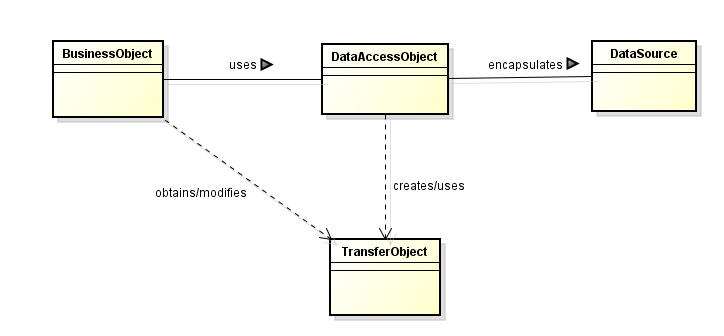
\includegraphics[width=\textwidth]{documenti/imgUML/DAO-pattern.png}
      \caption{Schema pattern DAO}
      \label{fig: archser}
    \end{figure}

\subsubsection{Dependency Injection}
Ogni lambda accetta in input le interfacce di cui necessita, le quali vengono istanziate da una funzione dedicata incaricata di fornire alla lambda i parametri corretti. Durante i test di unità, le classi mock vengono passate come parametri alle lambda.
\subsection{Schema del Database}
\begin{figure}[H]
      \centering
      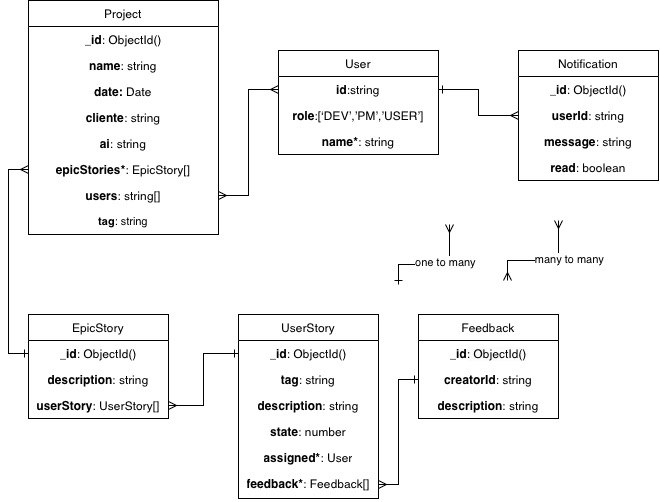
\includegraphics[width=\textwidth]{documenti/Screenshot manuale utente/UMLDB.png}
      \caption{Schema Database}
      \label{fig: archser}
    \end{figure}

Il Database di questa webApp è stato realizzato con Mongo DB. Lo schema rappresenta il diagramma del database dalla parte di backend. Alcune informazioni, infatti, per la parte di front-end sono superflue, oppure, al contrario, nel front-end saranno presenti alcune informazioni in più, ricavate dai dati salvati del database. Facendo così assicuriamo una chiara divisione delle responsabilità tra le diverse parti del sistema.\\
Vediamo in dettaglio lo schema, i valori indicati con * possono essere nulli:\\
\begin{itemize}
    \item \custombold{User}: è la tabella che salva i dati dell'utente\begin{itemize}
        \item \custombold{id}: è una stringa con gli id univochi dell'utente che corrisponde all'id che troviamo su Cognito;
        \item \custombold{role}: è un enum di stringhe che contiene il possibile ruolo degli utenti, DEV (sviluppatore), PM(Project Manager), User (cliente);
        \item \custombold{name}: è una stringa con il nome dell'utente;
    \end{itemize}
    \item \custombold{Project}: è la tabella che salva i datirelativi ai progetti\begin{itemize}
        \item \custombold{\_id}: è un oggetto apposito di MongoDB che rappresenta gli id univochi dei progetti;
         \item \custombold{tag}: è una stringa apposita per identificare e gestire meglio i progetti;
        \item \custombold{name}: è una stringa che contiene il titolo del progetto;
        \item \custombold{date}: è un Date che segna la data di creazine del progetto;
        \item  \custombold{cliente}: una stringa con il nome dell'azienda;
        \item \custombold{ai}: una stringa che specifica l'intelligenza artificiale da usare;
        \item \custombold{epicStories}: contiene un array di epic storyes collegate al progetto;
        \item \custombold{users}: è un array di utenti collegati al progetto, che possono lavorarci o visualizzare lo stato;
    \end{itemize}
    \item \custombold{EpicStory}: è la tabella che salva i dati delle epic story\begin{itemize}
        \item \custombold{\_id}: è un oggetto apposito di MongoDB che rappresenta gli id univochi della epic story;
        \item \custombold{description}: è una stringa che descrive cosa andrà a fare l'epic story;
        \item \custombold{userStory}: è un array di user story collegate all'epic story corrispondente;
    \end{itemize}
    \item \custombold{UserStory}: è la tabella che salva i dati delle user story\begin{itemize}
        \item \custombold{\_id}: è un oggetto apposito di MongoDB che rappresenta gli id univochi delle user story;
        \item \custombold{tag}: è una stringa univoca per ogni user story che serve per identificare meglio la user story e fare tutte le azioni possibili nel plugin;
        \item \custombold{description}: è una stringa che descrive cosa andrà a fare la user story;
        \item \custombold{state}: è un number che rappresenta lo stato della user story; nel nostro caso sarà 0=todo, 1=passing (ha passato tutti i test), 2=deleted (viene eliminata solo nel front end ma rimane nel database, solo se ha passato tutti i test);
        \item \custombold{assigend}: rappresenta lo sviluppatore a cui è stata assegnata la user story;
        \item \custombold{feedback}: un array di feedback che contengono i miglioramenti per l'intelligenza artificiale;
    \end{itemize}
    \item \custombold{Feedback}: è la tabella che salva i feedback inviati all'intelligenza artificiale\begin{itemize}
         \item \custombold{\_id}: è un oggetto apposito di MongoDB che rappresenta gli id univochi dei feedback;
        \item \custombold{creatorId}: è una stringa con l'id dell'utente che invia il feedback;
        \item \custombold{description}: è una stringa che descrive il messaggio da inviare all'IA per poter migliorare le prestazioni;
    \end{itemize}
    \item \custombold{Notification}: è la tabella che salva le notifiche tra i diversi utenti\begin{itemize}
        \item \custombold{\_id}: è un oggetto apposito di MongoDB che rappresenta gli id univochi per le notifiche;
        \item \custombold{userId}: è una stringa che contiene l'id del mittente;
        \item \custombold{message}: è una stringa con il corpo del messaggio;
        \item \custombold{read}: un booleano che segnala se la notifica è stata letta.
    \end{itemize}
\end{itemize}
Abbiamo utilizzato come id univoco l'id fornito automaticamente da MongoDB per facilitarci le operazioni e le query, dopo per facilitarne l'utilizzo nel front-end lo abbiamo reso una stringa. Mentre per l'id dell'utente abbiamo usato l'id fornito da Cognito.\\

Inserendo, poi, all'interno di ogni tabella i riferimenti che gli servono (come, ad esempio, dentro a progetto gli id delle epic story collegate) facilita il collegamento e l'elaborazione dei dati, anche se richiede un controllo in più nella fase di inserimento.

\subsection{Documentazione API}
In questa sezione è descritta ad alto livello la libreria creata per comunicare con l’applicazione, fornendo una panoramica delle API disponibili comprensiva di una breve
descrizione della loro funzionalità e suddivise per GET e POST.

\begin{center}
\begin{tabular}{|P{7cm}| P{10cm}|}
\hline
\rowcolor{Blue}
Lambda & Descrizione \\
\hline
\rowcolor{LightBlue}
\multicolumn{2}{|c|}{GET} \\
\hline
\rowcolor{LighterBlue}
/getProgetti & Se l'utente è loggato recupera la lista di tutti i progetti a cui un utente fa parte. \\
\hline
\rowcolor{LightBlue}
/getProgetto & Dato un id ritorna il progetto relativo a quell'id. \\
\hline
\rowcolor{LighterBlue}
/getEpicStory & Ottiene i dettagli di una specifica epic story. \\
\hline
\rowcolor{LightBlue}
/getUserStory & Recupera le informazioni relative a una user story specifica. \\
\hline
\rowcolor{LighterBlue}
/getUserStoryByTag & Tramite il tag recupera l'User story relativa. \\
\hline
\rowcolor{LightBlue}
/getAssignedUserStory & Recupera l'User story assegnata all'utente. \\
\hline
\rowcolor{LighterBlue}
/getNotifications & Recupera le notifiche per l'utente attuale. \\
\hline
\rowcolor{LightBlue}
/bedrock & Fornisce dati di base per il sistema (non specificato). \\
\hline
\rowcolor{LighterBlue}
/getProgetto & Recupera un progetto secondo un id. \\
\hline
\rowcolor{LightBlue}
/getProgettoByTag & Recupera un progetto tramite il tag. //
\hline
\multicolumn{2}{|c|}{POST} \\
\hline
\rowcolor{LighterBlue}
/addProgetto & Aggiunge un nuovo progetto al sistema. \\
\hline
\rowcolor{LightBlue}
/addEpicStory & Crea una nuova Epic story nel progetto specificato. \\
\hline
\rowcolor{LighterBlue}
/addUserStory & Crea una nuova User story nel progetto specificato. \\
\hline
\rowcolor{LightBlue}
/acceptInvite & Accetta un invito per un progetto. \\
\hline
\rowcolor{LighterBlue}
/invite & Invia un invito a un utente per unirsi a un progetto. \\
\hline
\rowcolor{LightBlue}
/assignDev & Assegna uno sviluppatore a una specifica user story. \\
\hline
\rowcolor{LighterBlue}
/setUnitTest & Imposta un test unitario per una funzionalità specifica. \\
\hline
\rowcolor{LightBlue}
/setUserStoryState & Imposta lo stato di avanzamento della User story. \\
\hline
\rowcolor{LighterBlue}
/readNotifications & Contrassegna le notifiche come lette. \\
\hline
\rowcolor{LightBlue}
/insertFeedback & Registra il feedback inviato dall'utente. \\
\hline
\rowcolor{LighterBlue}
/login & Permette a un utente di effettuare il login nel sistema. \\
\hline
\rowcolor{LightBlue}
/change\_password & Cambia password dell'utente. \\
\hline
\rowcolor{LighterBlue}
/register & Registra un nuovo utente nel sistema. \\
\hline
\end{tabular}
\captionof{table}{Lista delle Lambda}
\label{tab:lambda}
\end{center}
\subsection{Architettura del Plugin}
Il plugin di VSCode è stato sviluppato seguendo un approccio ad oggetti.\\
Di seguito il diagramma delle classi, e la lista dei loro attributi e metodi.
\begin{figure}[H]
    \centering
    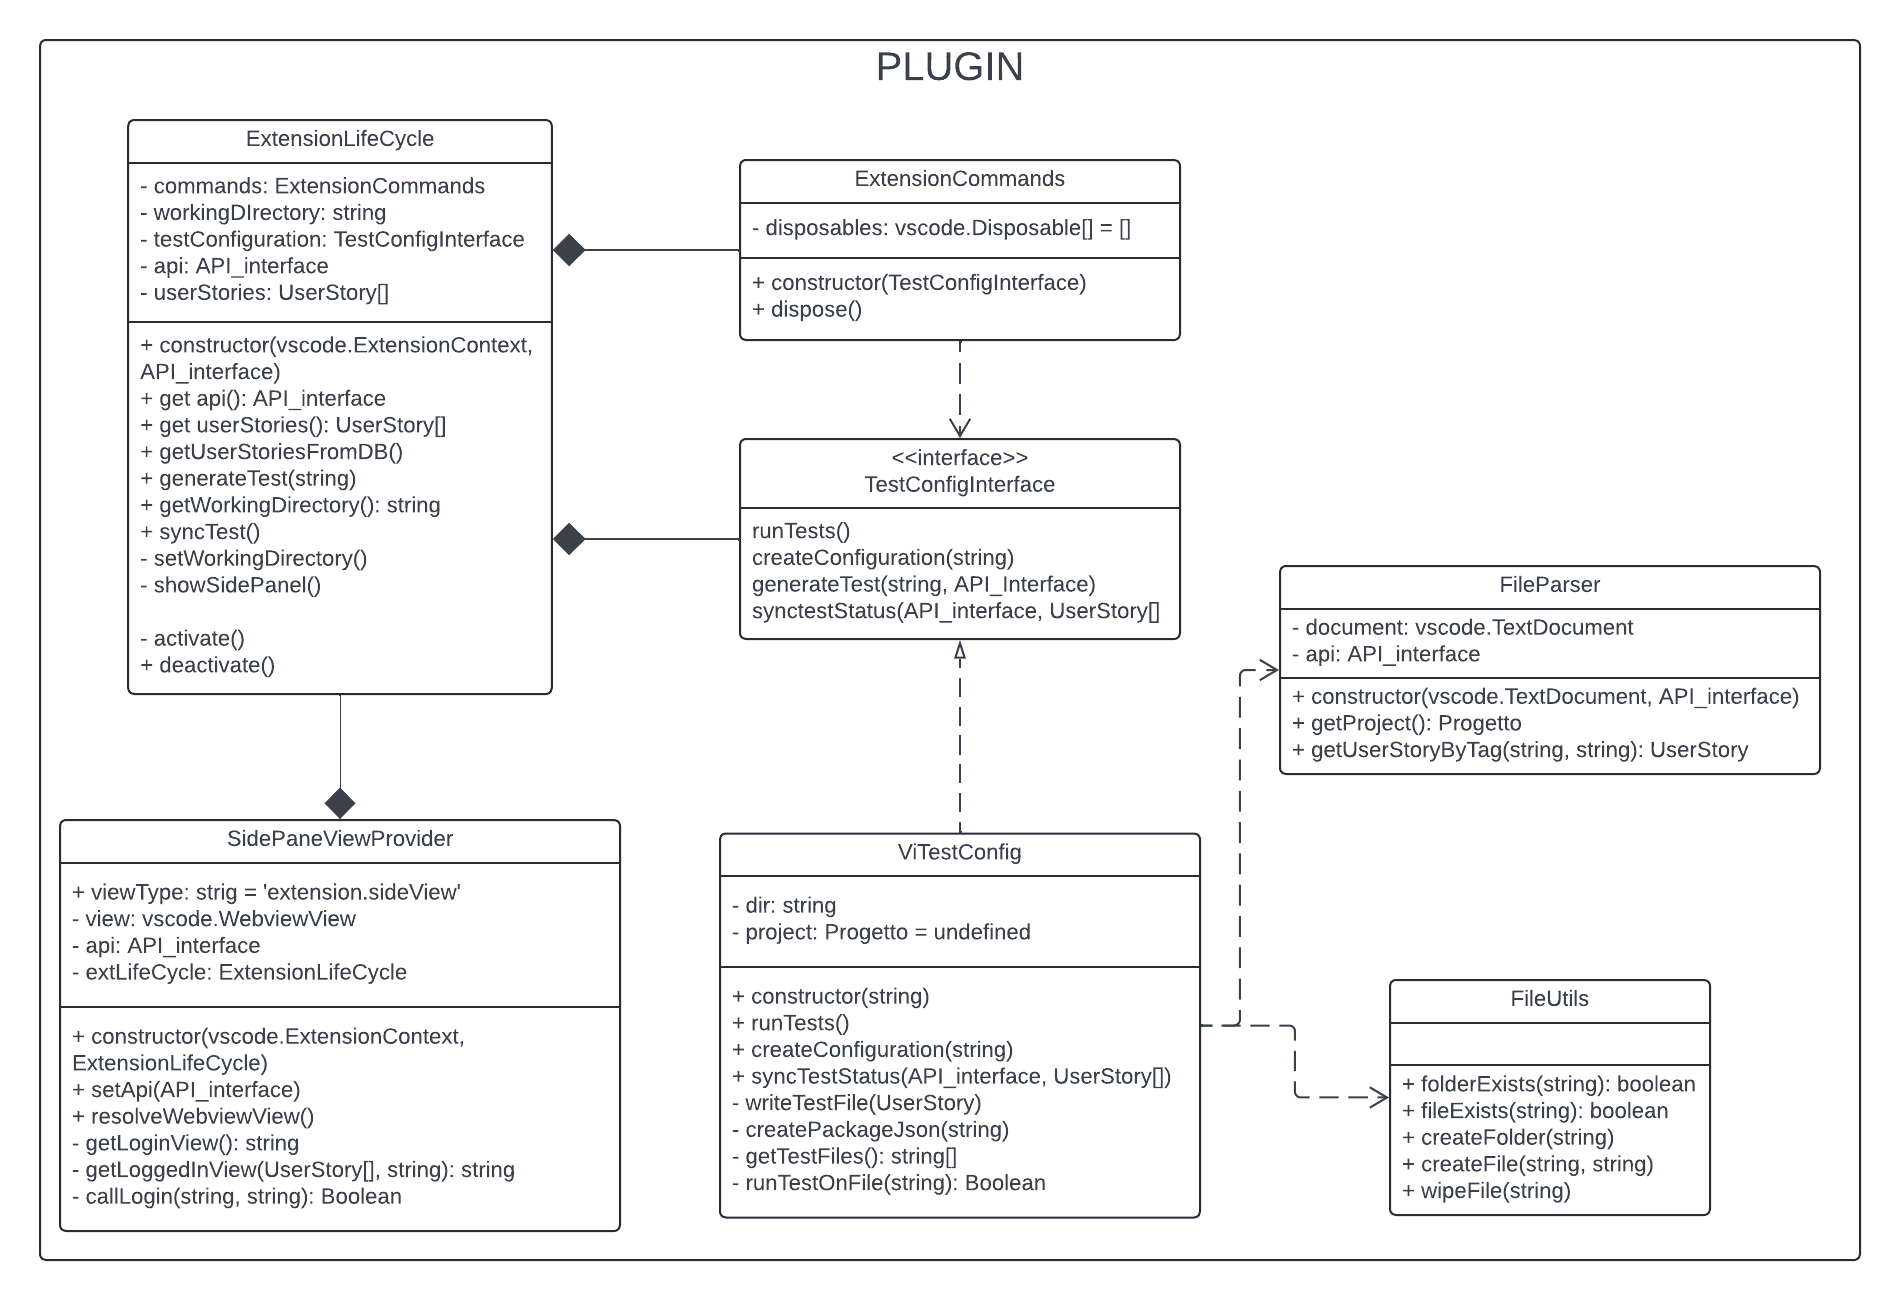
\includegraphics[width=\textwidth]{documenti/imgUML/plugin_class_diagram.png}
    \caption{Diagramma delle classi del Plugin}
    \label{fig:enter-label}
\end{figure}
\begin{itemize}
    \item \custombold{Classe: \textit{ExtensionLifeCycle}}
    \begin{itemize}
        \item Attributi
        \begin{itemize}
            \item  \custombold{commands: ExtensionCommands}: I comandi dell'estensione;
            \item \custombold{workingDirectory: string}: La cartella dove si sta lavaronado;
            \item \custombold{testConfiguration: TestConfigInterface}: L'oggetto che gestisce la configurazione dei test;
            \item \custombold{api: API\_Interface}: L'oggeto api della libreria, che gestisce le chiamate all'API;
            \item \custombold{userStories: UserStory[]}: L'array di user stories assegnate all'utente che utilizza l'estensione;
        \end{itemize}
        \item Metodi
        \begin{itemize}
            \item \custombold{constructor(vscode.ExtensionCommands, API\_interface)}: Costruisce un oggetto ExtensionLyfeCycle, prendendo il contesto dell'estensione e un oggetto API\_interface;
            \item \custombold{get api(): API\_interface}: Getter per l'attributo api;
            \item \custombold{get userStories(): UserStory[]}: Getter per l'attributo userStories;
            \item \custombold{getUserStoriesFromDB$()$}: Per un utente loggato all'interno dell'estensione, recupera tramite chiamata ad api le user stories a lui assegnate e le assegna all'attributo \textit{UserStories};
            \item \custombold{generateTest(string)}: Genera i test una data user story a partire dal suo tag;
            \item \custombold{getWorkingDirectory: string}: Restituisce il path assoluto della cartella di lavoro;
            \item \custombold{syncTest()}: Sincronizza i risultati dei test con il database, modificando il campo \textit{state} della user story;
            \item \custombold{setWorkingDirectory()}: Imposta la cartella di lavoro tramite pop-up di sistema;
            \item \custombold{showSidePanel()}: Renderizza il pannello laterale dell'estensione;
            \item \custombold{activate()}: Attiva l'estensione;
            \item \custombold{deactivate()}: Disattiva l'estensione;
        \end{itemize}
    \end{itemize}
        \item \textbf{Classe: \textit{ExtensionCommands}}
    \begin{itemize}
        \item Attributi
        \begin{itemize}
            \item \custombold{disposables: vscode.Disposable[] = []}: Array che contiene i comandi registrati;
        \end{itemize}
        \item Metodi
        \begin{itemize}
            \item \custombold{constructor(TestConfigInterface)}: Costruisce un oggetto della classe a partire da una TestConfifInterface;
            \item \custombold{dispose()}: Elimina i comandi quando un oggetto ExtensionCommand viene distrutto;
        \end{itemize}
    \end{itemize}
        \item \textbf{Interfaccia: \textit{TestConfigInterface}}
    \begin{itemize}
        \item Metodi
        \begin{itemize}
            \item \custombold{runTests()}: Esegue i test relativi alle user stories;
            \item \custombold{createConfiguration(string)}: Crea i file di configurazione nella cartella di lavoro, prendendo il suo path in input;
            \item \custombold{generateTest(string, API\_Iterface)}: Genera i test nella cartella di lavoro, prendendo in input il suo path;
            \item \custombold{syncTestStatus(API\_Interface, UserStory[])}: Sincronizza lo stato delle user stories in base ai risultati dei test;
        \end{itemize}
    \end{itemize}
        \item \textbf{Classe \textit{VitestConfig}}
    \begin{itemize}
        \item Attributi
        \begin{itemize}
            \item \custombold{dir: string} Rappresenta la cartella dove vengono generati i test;
            \item \custombold{project: Progetto = undefined} Rappresenta il progetto sul quale l'utente sta lavorando;
        \end{itemize}
        \item Metodi
        \begin{itemize}
            \item \custombold{constructor(string)}: Costruisce una nuova configurazione, e imposta dir alla cartella di lavoro;
            \item \custombold{runTests()}: Esegue i test relativi alla user story;
            \item \custombold{createConfiguration(string)}:Crea i file di configurazione nella cartella di lavoro, prendendo in input il suo path;
            \item \custombold{syncTestStatus(API\_Interface, UserStory[])}: Sincronizza lo stato delle user stories in base ai risultati dei test;
            \item \custombold{writeTestFile(UserStory)}: Genera un nuovo file di test per la usertory;
            \item \custombold{createPackageJson(string)}: Crea il file di configurazione package.json nella cartella passata in input;
            \item \custombold{getTestFiles(): string[]}: Restituisce un array di string, dove ognuna di esse è il path ad un file di test;
            \item \custombold{runTestOnFile(string): Boolean}: Dato il path ad un file di test, esegue il file. Restituisce \textit{true} se tutti i test passano, altrimenti restituisce \textit{false};
        \end{itemize}
    \end{itemize}
        \item \textbf{Classe: \textit{SidePanelViewProvider}}
    \begin{itemize}
        \item Attributi
        \begin{itemize}
            \item \custombold{viewType: string = 'extension.sideView'}: Nome della view, utilizzato per identificarla nel file di configurazione package.json del plugin;
            \item \custombold{view: vscode.WebviewView}: Contiene il codice per renderizzare la vista;
            \item \custombold{api: API\_Interface}: Istanza di un oggetto api utilizzata per fare le chiamate all'API;
            \item \custombold{extLifeCycle: ExtensionLifeCycle}: Oggetto ExtensionLifeCycle, contentente le funzionalità e i dati relativi all'istanza della estensione attiva;
        \end{itemize}
        \item Metodi
        \begin{itemize}
            \item \custombold{constructor(vscode.ExtensionContext, ExtensionLifeCycle}: Costruice un nuovo oggetto, a partire dal contesto dell'estensione. Imposta il campo extLyfeCycle;
            \item \custombold{setApi(API\_Interface)}: Setter per il campo api;
            \item \custombold{resolveWebView(vscode.WebviewView, vscode.WebviewViewResolveContext,} \\ \custombold{vscode.CancellationToken)}: Risolve una webView;
            \item \custombold{getLoginView: string}: Restituisce il codice necessario a renderizzare la pagina di login;
            \item \custombold{getLoggedInView(UserStory[], string): string}: Restituisce il codice per renderizzare la vista di un utente loggato. Mostra le user story a lui assegnate, un pulsante per ciascuna per generare i test, ed un pulsante generale per sincronizzare lo stato delle user story con il database;
            \item \custombold{callLogin(string, string): Boolean}: Prendendo in input email e password, gestisce la chiamata al login;
        \end{itemize}
    \end{itemize}
        \item \textbf{Classe: \textit{FileParser}}
    \begin{itemize}
        \item Attributi
        \begin{itemize}
            \item \custombold{document: vscode.TextDocument}: Il documento attivo, dove si esegue il parsing;
            \item \custombold{api: API\_Interface}: L'oggetto api che gestisce le chiamate ad API Gateway;
        \end{itemize}
        \item Metodi
        \begin{itemize}
            \item \custombold{constructor(vscode.TextDocument, API\_Interface)}: Costruisce un oggetto FileParser inizializzando tutti i suoi campi dati;
            \item  \custombold{getProject(): Progetto}: Restituisce il progetto relativo al file, recuperato dal tag sulla prima riga del file;
            \item  \custombold{getUserStoryByTag(string, string)}: Dato il tag di una userstory, se è presente il suo tag nel file, la restituisce;
        \end{itemize}
    \end{itemize}
        \item \textbf{Classe: \textit{FileUtils}}
    \begin{itemize}
        \item Metodi
        \begin{itemize}
            \item \custombold{folderExists(string): Boolean}: Dato un path di una cartella, verifica se esiste;
            \item \custombold{fileExists(string): Boolean}: Dato un path di un file, verifica se esiste;
            \item \custombold{createFolder(string)}: Crea una cartella nel path passato in input;
            \item \custombold{createFile(string, string)}: Crea un file a partire dal path e dal contenuto passati in input;
            \item \custombold{wipeFile(string)}: Svuota il file al path passato in input;
        \end{itemize}
    \end{itemize}
\end{itemize}
\subsection{Architettura della libreria}
Per raggruppare alcune funzionalità utili sia nel frontend che nel plugin, è stata sviluppata una libreria. Di seguito è presente il suo diagramma delle classi, ed una descrizione della sua struttura.
\begin{figure}[H]
    \centering
    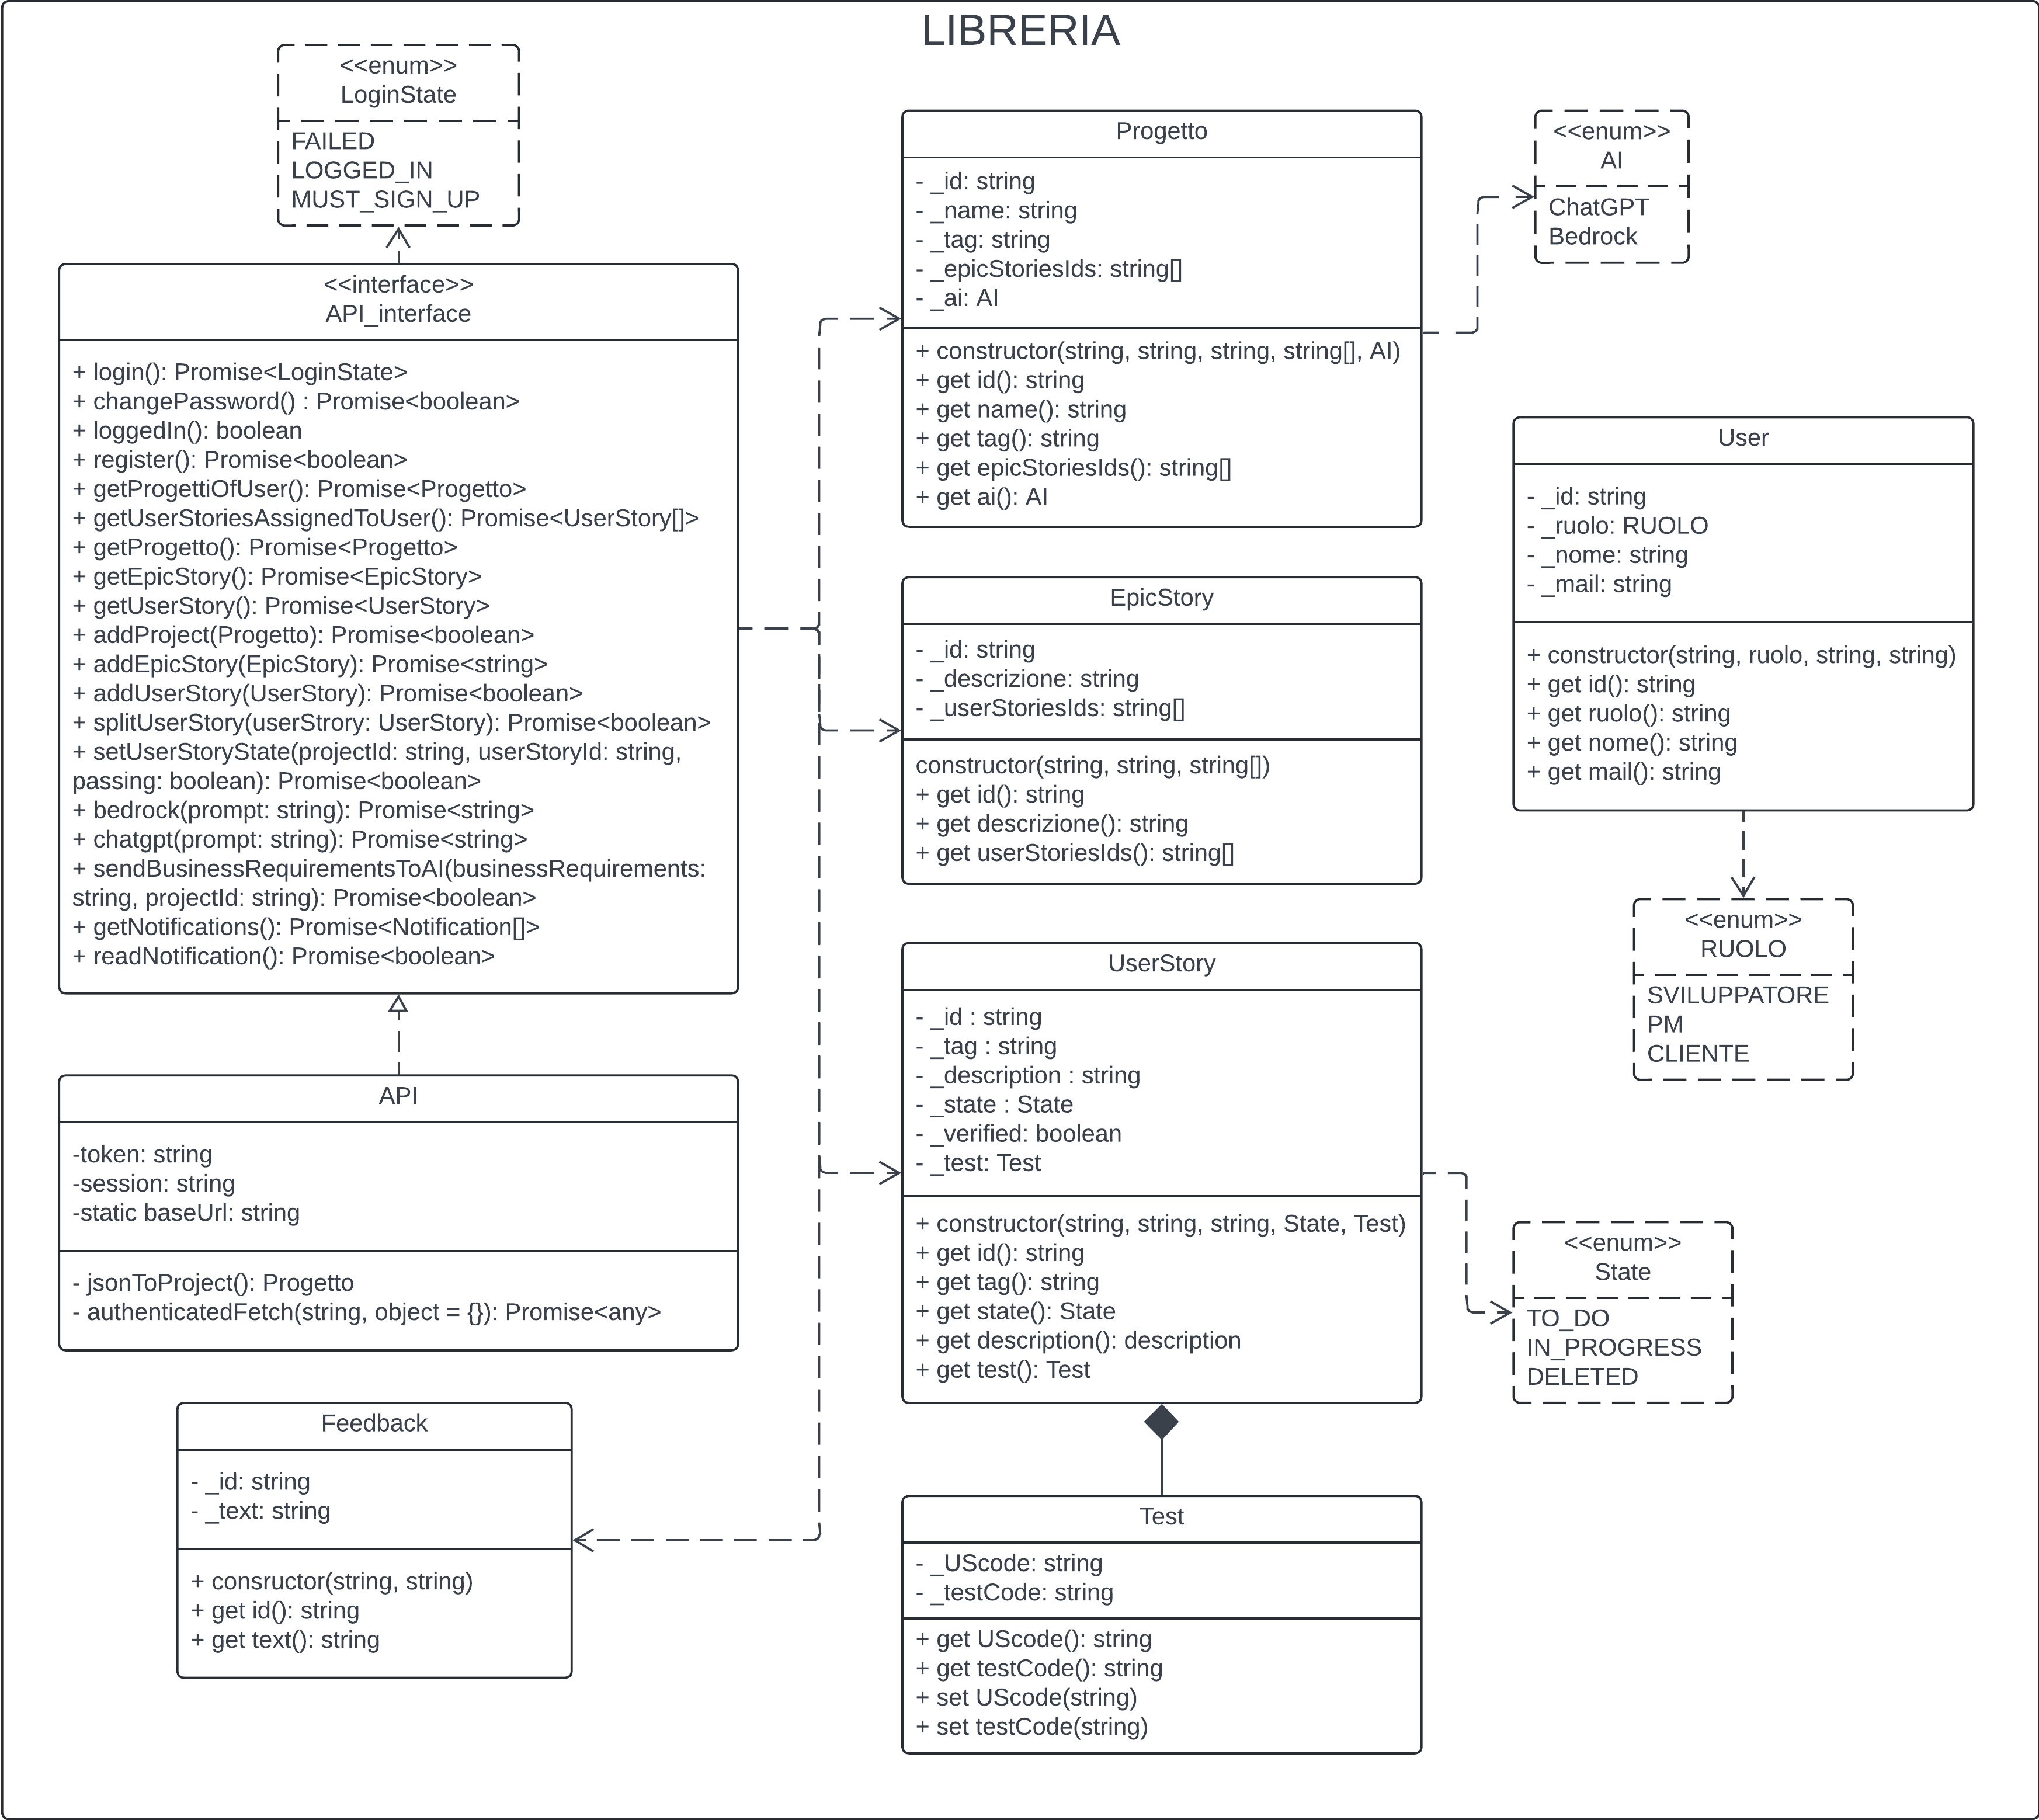
\includegraphics[width=\textwidth]{documenti/grafici/libreria_class_diagram.png}
    \caption{Diagramma delle classi della Libreria}
    \label{fig:enter-label}
\end{figure}
\begin{itemize}
    \item \textbf{Classe: \textit{Progetto}}  \begin{itemize}
        \item Attributi
        \begin{itemize}
        \item \custombold{\_id: string}: L\'id del progetto;
    	\item \custombold{\_name: string}: Il nome del proggetto;
    	\item \custombold{\_epicStoriesIds: string[]}: Le epic stoy che compongono il progetto;
    	\item \custombold{\_ai: AI} L'intelligenza artificiale da utilizzare per il progetto;
        \end{itemize}
        \item Metodi
        \begin{itemize}
            \item \custombold{constructor(project: ProjectData)} Costruisce un oggetto Progetto prendendo il contesto del project data;
            \item \custombold{get id(): string}: Getter per l'id;
            \item \custombold{get name(): string}: Getter per il nome del progetto;
            \item \custombold{get epicStoriesIds(): string[]}: Getter per la lista di epic story;
            \item \custombold{get ai(): AI}: Getter per l'intelligenza artificiale da usare;
        \end{itemize}
    \end{itemize}
\item \textbf{Classe: \textit{EpicStory}}  \begin{itemize}
        \item Attributi
        \begin{itemize}
        \item \custombold{\_id: string}: L\'id dell\'epic story;
    	\item \custombold{\_descrizione: string}: La descrizione di cosa deve fare l'epic story;
    	\item \custombold{\_userStoriesIds: string[]}: Le user stoy che compongono la specifica epic story;
        \end{itemize}
        \item Metodi
        \begin{itemize}
            \item \custombold{constructor(epic: EpicData)} Costruisce un oggetto EpicStory prendendo il contesto di EpicData;
            \item \custombold{get id(): string}: Getter per l'id;
            \item \custombold{get descrizione(): string}: Getter per la descrizione della epic story;
            \item \custombold{set descrizione(descrizione: string): void}: Setter per la descrizione della epic story;
            \item \custombold{get userStoriesIds(): string[]}: Getter per la lista di epic story;
        \end{itemize}
    \end{itemize}

    \item \textbf{Classe: \textit{UserStory}}  \begin{itemize}
        \item Attributi
        \begin{itemize}
            \item \custombold{\_id: string}: L'id dell'user story;
            \item  \custombold{\_tag: string}: Il tag univoco della user story;
    	\item \custombold{\-description: string}: La descrizione di cosa deve fare l'user story;
            \item  \custombold{\_state: State}: un numero che rappresenta 0 se To\_DO, 1 se IN\_Progress o 2 se DELETED per lo stato della user story;
            \item \custombold{\_verified:boolean}: per veedre se il codice scritto nel pluggin ha passato tutti i test;
            \item \custombold{\_test: Test}: contiene le informazioni per la creazione del test della user story;

        \end{itemize}
        \item Metodi
        \begin{itemize}
            \item \custombold{constructor(user: UserData)} Costruisce un oggetto UserStory prendendo il contesto di UserData;
            \item \custombold{get id(): string}: Getter per l'id;
            \item \custombold{get tag(): string}: Getter per il tag;
            \item \custombold{get verified(): boolean}: Getter per lo stato di verifica;
            \item \custombold{get state(): State}: Getter per lo stato della user story;
            \item \custombold{get description(): string}: Getter per la descrizione della user story;
            \item \custombold{get test(): Test}: Getter per il test automatico della user story;
            \item \custombold{set tag(theTag: string): void}: Setter per il tag;
            \item \custombold{set description(description: string):}: Setter per la descrizione della user story;
            \item \custombold{set state(state: State): void}: Setter per lo stato della user story;
            \item \custombold{set verified(verified: boolean): void}: Setter per la verifica;
            \item \custombold{set test(test: Test): void}: Setter per il test;

        \end{itemize}
    \end{itemize}

    \item \textbf{Classe: \textit{User}}  \begin{itemize}
        \item Attributi
        \begin{itemize}
            \item \custombold{\_id: string}: L'id dell'utente;
            \item  \custombold{\_ruolo: RUOLO}: Il ruolo dell'utente che puo' essere: 'PM', 'CLIENTE' o 'SVILUPPATORE';
    	\item \custombold{\_nome: string}: Il nome dell'utente;
            \item  \custombold{\_mail: string}: la mail dell'utente;
        \end{itemize}
        \item Metodi
        \begin{itemize}
            \item \custombold{get id(): string}: Getter per l'id;
            \item \custombold{get ruolo(): RUOLO}: Getter per il RUOLO;
            \item \custombold{get nome(): string}: Getter per il nome dell'utente;
            \item \custombold{get mail(): string}: Getter per la mail;

        \end{itemize}
    \end{itemize}

    \item \textbf{Classe: \textit{Feedback}}  \begin{itemize}
        \item Attributi
        \begin{itemize}
            \item \custombold{\_id: string}: L'id dell'feedback;
            \item  \custombold{\_text: string}: Iltesto del feedback;
        \end{itemize}
        \item Metodi
        \begin{itemize}
            \item \custombold{get id(): string}: Getter per l'id;
            \item \custombold{get text(): string}: Getter per il testo;

        \end{itemize}
    \end{itemize}

    \item \textbf{Classe: \textit{Test}}  \begin{itemize}
        \item Attributi
        \begin{itemize}
            \item \custombold{\_UScode : string}: L'id della user story per fare il test;
            \item  \custombold{\_testCode: string}: Il codice del test;
        \end{itemize}
        \item Metodi
        \begin{itemize}
            \item \custombold{constructor(code: string)}: Costruttore del test che prende il codice;
            \item \custombold{get UScode(): string}: Getter per il codice della user story;
            \item \custombold{get testCode(): string}: Getter per il codice del test;

        \end{itemize}
    \end{itemize}
    
       \item \textbf{Interfaccia: \textit{API\_Interface}}
    \begin{itemize}
        \item Metodi
        \begin{itemize}
            \item \custombold{loggedIn(): Boolean}: Restituisce true se l'utente è loggato, false altrimenti;
            \item  \custombold{login(string, string): Promise<LoginState>}: Dati email e password, effettua il login, restitusce lo stato di login;
            \item  \custombold{register(string, string): Promise<boolean>}: Dati email e password, registra un nuovo utente. Restituisce true se la registrazione è avvenuta con successo, false altrimenti;
            \item \custombold{changePassword(string, password):Promise<boolean>}: Data email e nuova password, cambia la password di un utente;
            \item \custombold{getProgettiOfUser(): Promise<Progetto[]>}: Restituisce un array contenente tutti i progetti a cui l'utente loggato è stato assegnato;
            \item \custombold{getUserStoriesAssignedToUser(): Promise<UserStory[]>}: Restituisce un array contenente tutte le user stories assegnate all'utente loggato;
            \item \custombold{getProgetto(projectId: string): Promise<Progetto>}: Dato il suo id, restituisce un progetto;
            \item \custombold{getEpicStory(epicId: string, projectId: string): Promise<EpicStory>}: Dato il suo id, restituisce una epic story;
            \item \custombold{getUserStory(userStoryId: string,  projectId: string): Promise<UserStory>}: Dato il suo id, restituisce una user story;
            \item \custombold{addProject(progetto: Progetto): Promise<boolean>}: Aggiunge un progetto al database;
            \item \custombold{addEpicStory(epic: EpicStory, projectId: string): Promise<string>}: Aggiunge una epic story al database;
            \item \custombold{addUserStrory(userStory: UserStory, projectId: string, epicStoryId: string): Promise<boolean>}: Aggiunge una user story al database;
            \item \custombold{splitUserStory(userStrory: UserStory): Promise<boolean>}: Data una user story troppo ampia, la divide in multiple user story;
            \item \custombold{setUserStoryState(projectId: string, userStoryId: string, passing: boolean): Promise<boolean>}: Modifica lo stato di una user story;
            \item \custombold{AI(prompt: string): Promise<string>}: Invia alla AI un prompt, e ne ritorna la risposta;
            \item \custombold{sendBusinessRequirementsToAI(businessRequirements: string, projectId: string):}\\ \custombold{Promise<boolean>}: Invia all'intelligenza artificiale selezionata per il progetto i requisiti di business;
            \item \custombold{getNotifications(): Promise<Notification[]>}: Restituisce un array di notifiche contenente tutte le notifiche invita all'utente loggato;
            \item \custombold{readNotification(string): Promise<boolean>}: Segna una notifica come letta;
        \end{itemize}
    \end{itemize}
    \item \textbf{Classe: \textit{API}}  \begin{itemize}
        \item Attributi
        \begin{itemize}
            \item \custombold{token: string}: Il token d'accesso per poter fare richieste all'API;
            \item  \custombold{session: string}: Identificatore di sessione utilizzato per mantenere lo stato tra diverse richieste dall'utente all'API;
            \item  \custombold{baseUrl: string}: Endpoint di base per l'API;
        \end{itemize}
        \item Metodi\\
        Oltre a tutti i metodi implementati richiesti dall'interfaccia abbiamo:
        \begin{itemize}
            \item \custombold{jsonToProject(object): Progetto }: Dato un progetto in formato json, restituisce un oggetto Progetto della libreria;;
            \item \custombold{async authenticatedFetch(string,object = {}):Promise<any>}: Per un utente loggato, esegue una fetch passando come header il token di autorizzazione.;
        \end{itemize}
    \end{itemize}
    
\end{itemize}

\section{Requisiti soddisfatti}
In questa sezione è riportata, dal documento di \textit{Analisi dei Requisiti 2.0.0} e seguendo le convenzioni lì illustrate, il soddisfacimento dei requisiti.

\begin{center}
    \begin{tabular}{|P{2cm}| P{10cm}| P{4cm}|}
    \rowcolor{Blue} 
\hline
Codice & Descrizione & Stato  \\ 
\rowcolor{LightBlue}
\hline
ROF1 & Accesso a web app tramite login composto da email e password. & Soddisfatto \\ 
\rowcolor{LighterBlue}
\hline
ROF2& Scrittura di richieste di business tramite box testuale da web app. & Soddisfatto\\ 
\rowcolor{LightBlue}

\hline
ROF3& Invio delle richieste di business da web app. & Soddisfatto\\
\hline
\rowcolor{LighterBlue}
ROF4& Visualizzazione andamento sviluppo richieste tramite barra di completamento basata sulla percentuale di user stories completate. & Soddisfatto\\
\rowcolor{LightBlue}
\hline
ROF5 & Approvazione o rifiuto del risultato relativo all'implementazione di una user story. & Soddisfatto \\
\hline
\rowcolor{LighterBlue}
RDF6 &  Ricezione notifiche quando user story completata. & Soddisfatto\\
\hline
\rowcolor{LightBlue}
ROF7 &  Funzionalità di tag nel plug-in.  & Soddisfatto\\
\hline
\rowcolor{LighterBlue}
ROF8 & Lista di user stories assegnate da Project Manager sia su web app che su plug-in. & Soddisfatto \\
\hline
\rowcolor{LightBlue}
RDF9 & Ricezione notifica su web app quando nuova user story è assegnata dal Project Manager. & Soddisfatto\\
\hline
\rowcolor{LighterBlue}
ROF10 & Invio del codice sviluppato a IA per richiesta verifica.& Soddisfatto\\
\hline
\rowcolor{LightBlue}
ROF11 & Visualizzazione user stories generate da IA.  &Soddisfatto\\
\hline
\rowcolor{LighterBlue}
ROF12& Invio di feedback sulle user stories generate all'IA.& Soddisfatto \\
\hline
\rowcolor{LightBlue}
ROF13&Suddivisione delle user stories troppo grandi.  & Soddisfatto\\
\hline
\rowcolor{LighterBlue}
ROF14 & Assegnazione user stories agli sviluppatori.& Soddisfatto\\
\hline
\rowcolor{LightBlue}
RDF15 & Ricezione notifiche quando user story\textsubscript{G} viene generata in seguito a richiesta del cliente. & Non soddisfatto\\
\hline
\rowcolor{LighterBlue}
ROF16& Invio richiesta di modifiche relative a user stories a IA prima di approvazione. & Soddisfatto\\
\hline
\rowcolor{LightBlue}
ROF17&Visualizzazione andamento epic/user stories assegnate.& Soddisfatto\\
\hline
\rowcolor{LighterBlue}
ROF18& Creazione di un plug-in per VSCode.& Soddisfatto\\
\hline
\rowcolor{LightBlue}
RDF19& Creazione di un plug-in per XCode.& Non soddisfatto\\
\hline
\rowcolor{LighterBlue}
ROF20& I linguaggi supportati dal plug-in sono Typescript e Javascript. & Soddisfatto\\
\hline
\end{tabular}


    \begin{tabular}{|P{2cm}| P{10cm}| P{4cm}|}
\hline
\rowcolor{LightBlue}
RDF21 & Altri linguaggi che potrebbero essere supportati in futuro sono Kotlin\textsubscript{G} e Swift.& Non soddisfatto\\
\hline
\rowcolor{LighterBlue}
ROF22 & Gestione degli input (prevenzione da Injection Cross Site Scripting e sanificazione dell'input.) & Soddisfatto \\
\hline
\rowcolor{LightBlue}
ROQ1& Il progetto deve essere accessibile pubblicamente su GitHub o su un'altra repository pubblica. & Soddisfatto\\ 
\rowcolor{LightBlue}
\hline
ROQ2 & Il prodotto deve essere sviluppato conformemente a quanto stabilito nelle \textit{Norme Way of Working\textsubscript{G}}.& Soddisfatto \\ 
\rowcolor{LighterBlue}
\hline
ROQ3 & Deve essere effettuato il testing delle unità e dell'integrazione con una copertura minima dell'80\%.& Soddisfatto\\
\hline
\rowcolor{LightBlue}
ROQ4 & Deve essere fornita una documentazione completa sulle scelte implementative e progettuali effettuate. & Soddisfatto\\
\hline
\rowcolor{LighterBlue}
ROQ5& Deve essere fornito un manuale per l'utilizzo del prodotto. & Soddisfatto\\
\hline
\rowcolor{LightBlue}
ROQ6& Deve essere fornita una documentazione che compara la capacità di ChatGPT e quella di AWS Bedrock nell'interpretare del codice sorgente ed associare le user stories generate. & Soddisfatto\\
\hline
\rowcolor{LighterBlue}
ROQ7&  Deve essere fornita una documentazione che prova un'interpretazione corretta da parte dell'IA che si basa: sulle epic/user stories generate dall'IA, i test generati dall'IA, i criteri di accettazione delle epic/user stories forniti dal proponente. & Soddisfatto\\
\rowcolor{LightBlue}
\hline
ROV1& L'applicazione per l'interazione con la piattaforma dev'essere sviluppata attraverso l'uso di tecnologie web. & Soddisfatto\\ 
\hline
\rowcolor{LighterBlue}
ROV2& Le due IA utilizzate per l'analisi sono AWS Bedrock e ChatGPT. & Soddisfatto \\ 
\rowcolor{LightBlue}
\hline
RDV3& L'applicazione deve essere utilizzabile tramite browser (Chrome 123.0, Firefox 124.0, Safari 17.0) di dispositivi mobili(Android 14.0, iOS 17.0). & Non soddisfatto\\
\hline
\rowcolor{LighterBlue}
ROV4& Il front-end dell'applicazione verrà sviluppato in React. & Soddisfatto\\
\rowcolor{LightBlue}
\hline
ROV5& Ogni AWS Lambda-function deve essere sviluppata in Node.js.& Soddisfatto\\
\hline
\end{tabular}


    \begin{tabular}{|P{2cm}| P{10cm}| P{4cm}|}
\hline
\rowcolor{LighterBlue}
ROV6& Tutte le API devono essere integrate in AWS API-gateway.& Soddisfatto\\
\hline
\rowcolor{LightBlue}
ROV7& L'applicativo deve essere compatibile con il browser Google Chrome dalla versione 121. & Soddisfatto\\
\hline
\rowcolor{LighterBlue}
ROV8& L'applicativo deve essere compatibile con il browser Firefox dalla versione 122. & Soddisfatto\\
\hline
\rowcolor{LightBlue} 
ROV9 & L'applicativo deve essere compatibile con il browser Microsoft Edge dalla versione 121. & Soddisfatto\\
\hline
\rowcolor{LighterBlue}
ROV10 & Il plug-in deve essere compatibile con VSCode dalla versione 1.84.1 . & Soddisfatto\\
\hline
\rowcolor{LightBlue}
ROV11 &  L'accesso deve essere controllato da AWS Cognito, con autenticazione univoca. & Soddisfatto\\
\hline
\rowcolor{LighterBlue}
ROV12 & I ruoli devono essere definiti all'interno della piattaforma per evitare accessi non autorizzati. & Soddisfatto\\
\hline
\rowcolor{LightBlue}
ROV13 & Protezione delle informazioni trasmesse tra browser e server tramite protocollo SSL/TLS. & Soddisfatto\\
\hline
\end{tabular}
\captionof{table}{Tabella dei requisiti soddisfatti}
\label{tab:reqsodd}
\end{center}

\subsection{Resoconto dei requisiti soddisfatti}
\begin{center}
    \begin{tabular}{|P{7cm}| P{4cm}| P{4cm}|}
    \hline
    \rowcolor{Blue} 
    Tipologia requisito & Istanze & Totale soddisfatto\\
    \hline
    \rowcolor{LighterBlue}
    Requisito funzionale & 22 & 86,36\%\\
    \hline
    \rowcolor{LightBlue}
    Requisito obbligatorio & 36 & 100\% \\
\hline
\end{tabular}
\captionof{table}{Tabella di resoconto dei requisiti soddisfatti}
\label{tab:reqsoddrecap}
\end{center}


\end{document}